\documentclass[12pt]{article}
\usepackage[margin=1.0in]{geometry}
\usepackage{hyperref}
\usepackage{amsmath}
%\usepackage{amsmath}
\usepackage{graphicx}
% \usepackage[extendedchars]{grffile}
\usepackage{chngpage}
\usepackage{calc}


\title{Generation of milliCharged particles at the LHC}

\author{C. Campagnari, B. Marsh (UCSB), F. Golf (UNL)}

\begin{document}
\maketitle


\section{Introduction}
We discuss the MC generation of milliCharged
particles ($\zeta$) in $pp$ collisions at the LHC in the central rapidity
region. 
Except for Drell-Yan (DY), this is done in a few steps
\begin{enumerate}
\item Generate in various ways SM particles ($A$) that can decay as
  $A \to X \zeta^+ \zeta^-$
\item Keep track of the cross-section for SM production of $A$.
\item Calculate the branching ratio for $A \to X \zeta^+ \zeta^-$
  for milliCharge $Q=1$.  For different charges, it is easy to
  scale the branching ratio as $Q^2$.
\item Generate the $A \to X \zeta^+ \zeta^-$ decay with proper
  kinematics.
\item Save the ``event'' for further processing in a root file.
  \end{enumerate}
  


\section{Special (simplest) case: Drell-Yan}
The Drell-Yan process $pp \to \zeta^+ \zeta^-$ is generated with
the external model interface in MadGraph.  Note that we cannot use
SM $pp \to \ell^+ \ell^-$ with a different lepton mass
because the couplings of the $Z$ to
$\zeta$'s and leptons are different
(in our model $\zeta$'s are weak isospin
singlets\cite{Holdom}\cite{Haas:2014dda}).

Technically, this was achieved in MadGraph by simply modifying the mass and couplings
of the SM electron. The couplings are $\varepsilon e$ and $-\varepsilon e\tan\theta_W$ to
the $\gamma$ and $Z_0$, respectively, where $\varepsilon = Q/e$.

The $pp\to\zeta^+\zeta^-$ process is generated with up to 1 extra parton. This is not very 
relevant at lower masses since a large majority of events don't include an extra parton. At 
higher masses, however, it can increase cross section by $O$(20-30\%). The MadGraph
parameter \texttt{xqcut} is set to 0, but there still seems to be a 20 GeV cut on the $p_T$
of the extra parton.

We can't find a parameter to control this, but there appears to be a $\zeta^+\zeta^-$ invariant
mass cut of 2 GeV. Correspondingly, the cross section plateaus below $m_\zeta = 1$ GeV. This shouldn't
matter, however, as production from J/$\psi$, $\phi$, $\omega$, $\rho$, etc. is expected do dominate
at low masses.

A plot of DY cross section as a function of mass is shown along with the other production modes
in Fig. \ref{fig:total-rates}. Note that DY is handled specially here: while for the other modes
we require the mother particle to have $|\eta|<2$, this does not make sense for DY (unless there
is an extra parton produced, the $\eta$ of the ``mother'' is $\pm\infty$). Instead we have required
at least one mCP to have $|\eta|<1$. This threshold was chosen so that the probability of
an mCP pointing in the vicinity of the detector is similar between DY and the other modes, in order
to facilitate comparison of cross sections.



\section{List of non-DY processes}
\label{sec:list}

The main processes for  $A \to e^+ e^- X$ at the LHC are:
\begin{itemize}
    \item $\pi^0 \to e^+ e^- \gamma$  (BR=1.17\%, Dalitz decay)
    \item $\eta \to e^+ e^- \gamma$   (BR=0.7\%, Dalitz decay)
    \item $\eta' \to e^+ e^- \gamma$   (BR=5e-4, Dalitz decay)
    \item $\omega \to \pi^0 e^+ e^-$  (BR=8e-4, Dalitz decay)
    \item $\eta' \to \omega e^+ e^-$ (BR=2e-4, Dalitz decay)
    \item $\eta' \to \pi^+ \pi^- e^+ e^-$ (BR=2e-3, skip, see comment in Section~\ref{sec:bottom-line})
    \item $V \to e^+ e^-$ ($V$ = onia, $\phi$, $\rho$, $\omega$)
\end{itemize}

Note that if we are only interested in $\zeta$ masses above 100 MeV,
Dalitz decays of $\pi^0$ and decays of $\eta'$ into $\omega$
do not contribute.
In all cases the BR for $A \to \zeta^+ \zeta^- X$ can be obtained
by rescaling $A \to e^+ e^- X$ by a factor of $Q^2$ times an
additional mass-dependent factor.  In general this factor consists
of a phase space piece $\sqrt{1 - (2m_\zeta/m_A)^2}$ plus an additional
piece that arises from the matrix element.

Note also that among these processes, the paper~\cite{Haas:2014dda} that
proposed the milliqan experiment only included onia.  Furthermore
it is not clear that it included the $B \to \psi$ process, it
is not clear that it included $\psi(2S)$, $\Upsilon(2S)$,
and $\Upsilon(3S)$, and it imposed requirements $p_T > 6.5$ GeV (2 GeV)
on $J/\psi$ and $\Upsilon(1S)$, respectively.
The Letter of Intent~\cite{Ball:2016zrp} also mentions
$\Upsilon(2S)$ and $\Upsilon(3S)$, and it is possible that the latest
NSF proposal included even more processes.  In any case: here we make an
attempt to include as many processes as possible and to
remove $p_T$ requirements.


\section{Branching Ratios of non-DY processes (Q=1).}

\subsection{Dalitz BR}

The partial width for $A \to e^+ e^- \gamma$ can be written
as\cite{landsberg, bib:ulrik}:

\begin{equation}
\frac{d \Gamma}{d q^2} = \frac{2 \alpha}{3 \pi q^2}~~
(1+\frac{2m_e^2}{q^2})~~\sqrt{1 - \frac{4m_e^2}{q^2}}~~
(1 - \frac{q^2}{m_A^2})^3~~
|F(q^2)|^2 ~~
\Gamma(A \to \gamma \gamma) 
\label{dalitz1}
\end{equation}

\noindent where $m_A$ is the mass of $A$, $q^2$ is the mass-squared of the
$e^+e^-$ pair, 
and $F(q^2)$ is a form factor.  Note the $1/q^2$ factor that results
in a highly non-uniform invariant mass distribution sharply peaked at
low
values.
The form factor is such that $F(0)=1$ and for pions is usually
parametrized near $q^2=0$ as $F(q^2) = 1 + a \frac{q^2}{m_\pi^2}$ with
$a \approx 0.03$.  The form factor can also be estimated in the Vector
Dominance Model (VDM) as

\begin{equation}
  |F(q^2)|^2 = \frac{m^4_\rho + m^2_\rho \Gamma^2_\rho}{(m_\rho^2 - q^2)^2 + m^2_\rho \Gamma^2_\rho}
  \label{dalitz2}
\end{equation}

\noindent where $m_\rho$ and $\Gamma_\rho$ are the mass and width of the
$\rho$ meson.  The VDM model assumes that the decay proceeds through
$\pi^0 \to \gamma V^*, V^* \to e^+e^-$ and $V= \rho$ or $\omega$;
equation~\ref{dalitz2} neglects the difference between $\rho$ and $\omega$.

In the case of $A \to e^+ e^- X$, when $X$ is not $\gamma$, the
partial width can be written as 

\begin{equation}
\begin{split}
\frac{d \Gamma}{d q^2}  ~=~~~ & \frac{\alpha}{3 \pi q^2}~~
(1+\frac{2m_e^2}{q^2})~~\sqrt{1 - \frac{4m_e^2}{q^2}}~~ \cdot \\
& \left [ (1+\frac{q^2}{m_A^2-m_X^2})^2 - \frac{4
    m_A^2q^2}{(m_A^2-m_X^2)^2}\right ]^{3/2}~~
|F_{AX}(q^2)|^2 ~~
\Gamma(A \to X \gamma) 
\label{dalitz11}
\end{split}
\end{equation}

\noindent where $m_X$ is the mass of $X$, and the
transition
form factor $F_{AX}$ can also be approximated as in equation~\ref{dalitz2}.

For milliCharged particles, Dalitz decays branching ratios 
can be obtained by integrating equation~\ref{dalitz1} or~\ref{dalitz11}
from 
$q^2=4m^2_\zeta$ to the kinematical limit, substituting $m_\zeta$ for 
$m_e$, and rescaling by $Q^2$.
Some numerical results for $Q=1$ are given in Table~\ref{tab:dalitz1}.  Note the
sharp drop in branching ratios with mass.  This is due to the $1/q^2$ behavior.
The calculations
with the electron and muon masses are in excellent agreement with the PDG.



\begin{table}
  \begin{center}
    { \footnotesize
  \begin{tabular}{|c|c|c|c|c|c|}
    \hline
    $m_\zeta$ (MeV) & $\pi^0 \to \zeta \zeta \gamma$ & $\eta \to \zeta \zeta \gamma$
    & $\eta' \to \zeta \zeta \gamma$ & $\eta' \to \zeta \zeta \omega$
    & $\omega \to \zeta \zeta \pi^0$ \\ \hline \hline
  0.511 (=$m_e$)  & 1.17 e-2 & 6.6 e-3 & 4.6 e-4 & 1.8 e-4 & 7.6 e-4 \\
  PDG for ee  & ($1.17 \pm 0.04$)e-2 & ($6.9 \pm 0.4$)e-4 & ($4.7 \pm 0.3$)e-4  &
  ($2.0 \pm 0.4$)e-4  & ($7.7 \pm 0.6$)e-4 \\ \hline
  10              & 2.8 e-3  & 2.9 e-3 & 2.5 e-4 & 5.7 e-5 & 3.7 e-4 \\
  30              & 3.5 e-4  & 1.6 e-3 & 1.8 e-4 & 1.7 e-5 & 2.3 e-4 \\
  50              & 1.2 e-5  & 1.0 e-3 & 1.4 e-4 & 4.3 e-6 & 1.6 e-4 \\
  60              & 2.7 e-7  & 8.2 e-4 & 1.3 e-4 & 1.7 e-6 & 1.4 e-4 \\
  90              &         & 4.3 e-4 & 1.0 e-4 &        & 9.2 e-5 \\ \hline
  105.7 (=$m_\mu$)&         & 3.0 e-4 & 9.2 e-5 &         & 7.4 e-5 \\
  PDG for $\mu\mu$ &      & ($3.1 \pm 0.4$) e-4 & ($1.1 \pm 0.3$) e-4 & &
                      ($1.3 \pm 0.2$) e-4 \\ \hline
  150             &        & 8.9 e-5  & 6.8 e-5 &        & 3.7 e-5 \\
  200             &        & 1.2 e-5  & 4.8 e-5 &        & 1.5 e-5 \\
  250             &        & 1.0 e-7 & 3.2 e-5 &         & 3.6 e-6 \\
  400             &        &        & 5.6 e-7 &         &        \\ \hline 
  \end{tabular}
  }
  \caption{\protect Branching ratios for different Dalitz decay modes as 
    a function of $m_\zeta$ for $Q=1$ calculated 
    based on equations~\ref{dalitz1},~\ref{dalitz2}, and~\ref{dalitz11}. 
When possible we compare with 
  the values from the 2019 PDG.}
\label{tab:dalitz1}
  \end{center}
\end{table}

\subsection{Vector meson branching ratios}

  At lowest order the SM decay rate for $V \to \ell \ell$ is given
  by the Van Royen-Weisskopf formula\cite{VR1,VR2}:

  \begin{equation}
    \Gamma(V \to \ell \ell) = 4 \pi \alpha^2 \frac{f_V^2}{m_V} Q_q^2
    (1-4x_\ell^2)^{1/2} (1+2x_\ell^2)
    \end{equation}

  \noindent where $f_V$ is the vector decay constant, $m_V$ is the
  vector mass, $Q_q$ is the charge of the quark that makes up the meson,
  $x_\ell = m_\ell/m_V$, and $m_\ell$ is the lepton mass.

  \noindent Thus the ratio of BR for $V \to \zeta \zeta$ to $V \to ee$ is
  given by

  \begin{equation} 
    \frac{\Gamma(V \to \zeta \zeta)}{\Gamma(V \to ee)} = Q^2
    \frac{(1-4x_\zeta^2)^{1/2} (1+2x_\zeta^2)}{(1-4x_\ell^2)^{1/2} (1+2x_\ell^2)}
    \label{V1}
    \end{equation}

  \noindent where $x_\zeta = m_\zeta/m_V$, and $m_\zeta$ is the mass of $\zeta$.
  
  As a sanity check, we use equation~\ref{V1} to predict several $V \to \ell \ell$
  branching ratios and compare them with their PDG values, see Table~\ref{tab:VBR}.
  To be fair the tests with $\ell = \mu$ are not very powerful since
  $x_{\mu}^2 \approx x_{e}^2 \approx 0$.

  \begin{table}
    \begin{center}
      \begin{tabular}{|l|c|c|}
        \hline
        Decay mode & PDG BR value & Calculation \\
        \hline
        $\Upsilon(1S) \to \tau \tau$  & (2.6 $\pm$ 0.1)e-2 & (2.4 $\pm$ 0.1)e-2 \\
        $\psi(2S) \to \tau \tau$  & (3.1 $\pm$ 0.4)e-3 & (3.1 $\pm$ 0.0)e-3 \\
        $\phi \to \mu \mu$       & (2.9 $\pm$ 0.2)e-4  & (3.0 $\pm$ 0.0)e-4 \\  
        $\omega \to \mu \mu$ & (7.4 $\pm$ 1.8)e-5  & (7.3 $\pm$ 0.2)e-5 \\  
        $\rho \to \mu \mu$      & (4.6 $\pm$ 0.3)e-5  &  (4.7 $\pm$ 0.1)e-5 \\  
        \hline
      \end{tabular}
      \caption{Comparison of the PDG and calculated values od the $V \to \ell \ell$
        branching ratios.  The quoted uncertainty on the calculation reflects the uncertainty
        on the $V \to ee$ branching ratio.}
      \label{tab:VBR}
    \end{center}
  \end{table}
  \section{Generation of SM particles decaying into $\zeta^+ \zeta^-$}


  The key features of our approach are the following
\begin{itemize}
\item Use theory or published data, or some MC to generate $p_T$ distributions for SM
  particles
saved as histograms in ROOT files (Drell Yan is an exception, as discussed previously).
\item Sample the ROOT histograms to generate SM particles of a 
given $p_T$.
\item Pick azimuthal angles $\phi$ and pseudorapity $\eta$ in a
  limited 
  range, matched to the acceptance of milliqan.  The $\eta$
  distribution is assumed to be flat, see comments in
  Section~\ref{sec:bottom-line}.
\item Decay the SM particles into milliCharged particles. 
\item When possible, keep track of theoretical uncertainties.
\item In general it is sufficient to generate SM particles at low 
and moderate $p_T$ since that is where the cross-section is largest.
\end{itemize}

\subsection{J/$\psi$ and $\psi'$ from b-decays}
\label{sec:bpsi}
We use the tool available in \\
\href{http://www.lpthe.jussieu.fr/~cacciari/fonll/fonllform.html}
{http://www.lpthe.jussieu.fr/~cacciari/fonll/fonllform.html} \\
to
generate histograms of $p_T$ distributions (cross-sections) for charmonium from 
bottom decays, including theoretical 
uncertainties\cite{Cacciari:2012ny,Cacciari:2015fta}.  
See Figure~\ref{fig:bpsi} 

\begin{figure}
  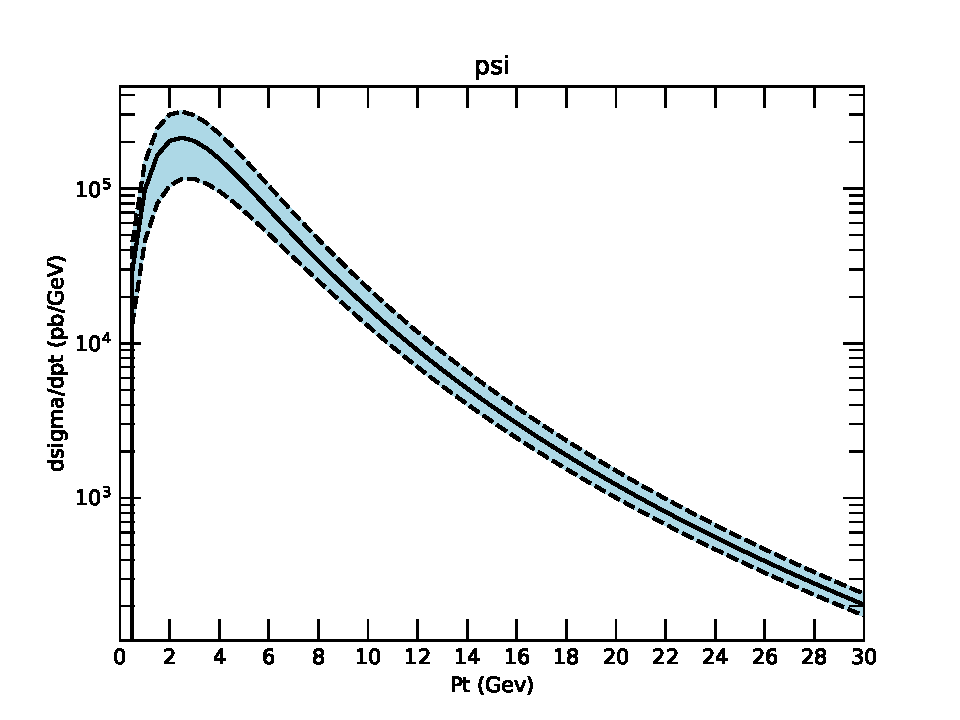
\includegraphics[width=0.48\linewidth]{../oniaFromB/psi.pdf}
  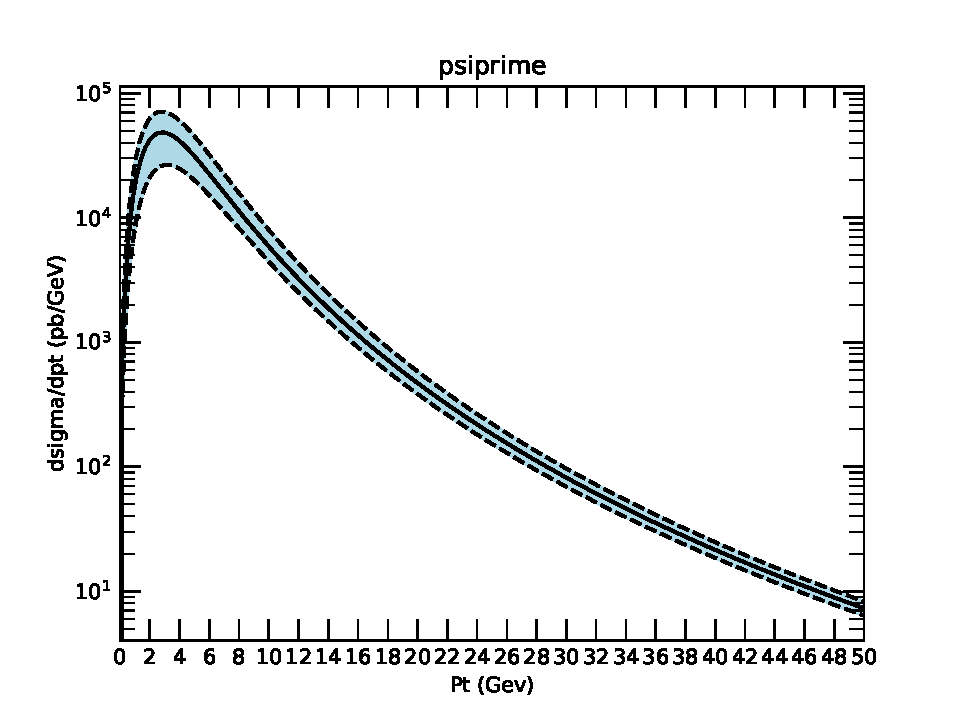
\includegraphics[width=0.48\linewidth]{../oniaFromB/psiprime.pdf}
  \caption{Transverse momentum distributions of J/$\psi$ (left) 
and $\psi'$ from bottom quark decays. Note: this is from a single $b$, 
multiply by two to include $\bar{b}$. The units are pb/GeV and the 
distributions 
are integrated over $|\eta|<1.0$.}
  \label{fig:bpsi}
\end{figure}

  
\subsection{Direct onia production}
\label{sec:onia}

\subsubsection{Direct bottonium}
\label{sec:upsilon}

There have been many measurement of the $p_T$ spectra od $\Upsilon$ in $pp$ collisions
at the LHC by CMS~\cite{Khachatryan:2010zg, Chatrchyan:2013yna, Khachatryan:2015qpa, Sirunyan:2017qdw},
Atlas~\cite{Aad:2011xv, Aad:2012dlq},
  and LHCb~\cite{Aaij:2018pfp, Aaij:2015awa, Aaij:2014nwa, Aaij:2013yaa, LHCb:2012aa}.
  The LHCb measurements are in the forward region.  The only measurement at 13 TeV
  in the central region is from CMS~\cite{Sirunyan:2017qdw}.  Unfortunately, it is limited
  to $p_T >$ 20 GeV.

  Due to the lack of 13 TeV data, initially we planned to use theoretical predictions
  as a basis of the $\Upsilon$ event generation.
  We contacted the theorists~\cite{Han:2014kxa}
  that provided the state-of-the art calculations used to
  confront the data in Reference~\cite{Sirunyan:2017qdw}.  We
  asked them to extend their predictions to lower $p_T$, unfortunately they claim that these
  are unreliable below 15 GeV.

\begin{figure}
\begin{adjustwidth}{-2cm}{-2cm}
\centering
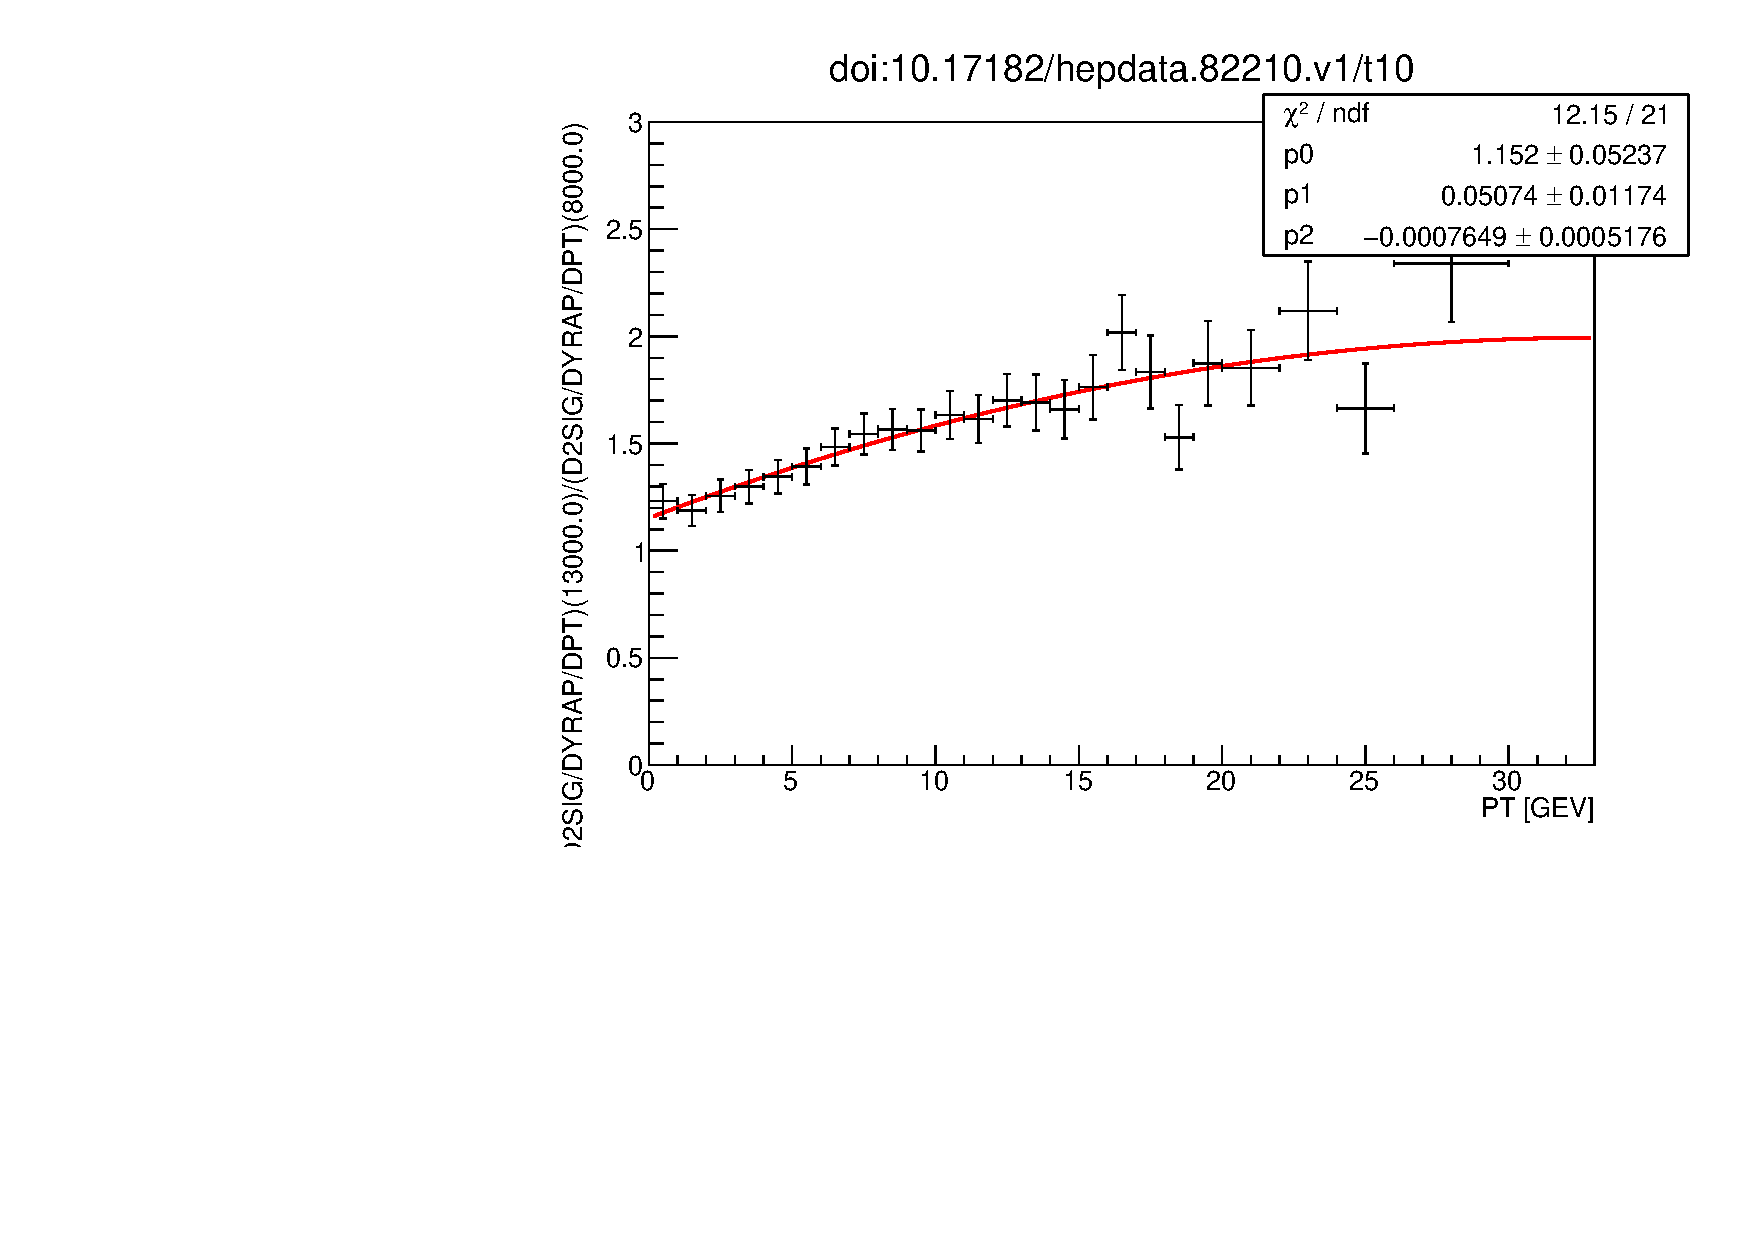
\includegraphics[width=0.32\linewidth]{../oniaDirect/LHCB-13-TeV/ups1s-13to7eta20to25.pdf}
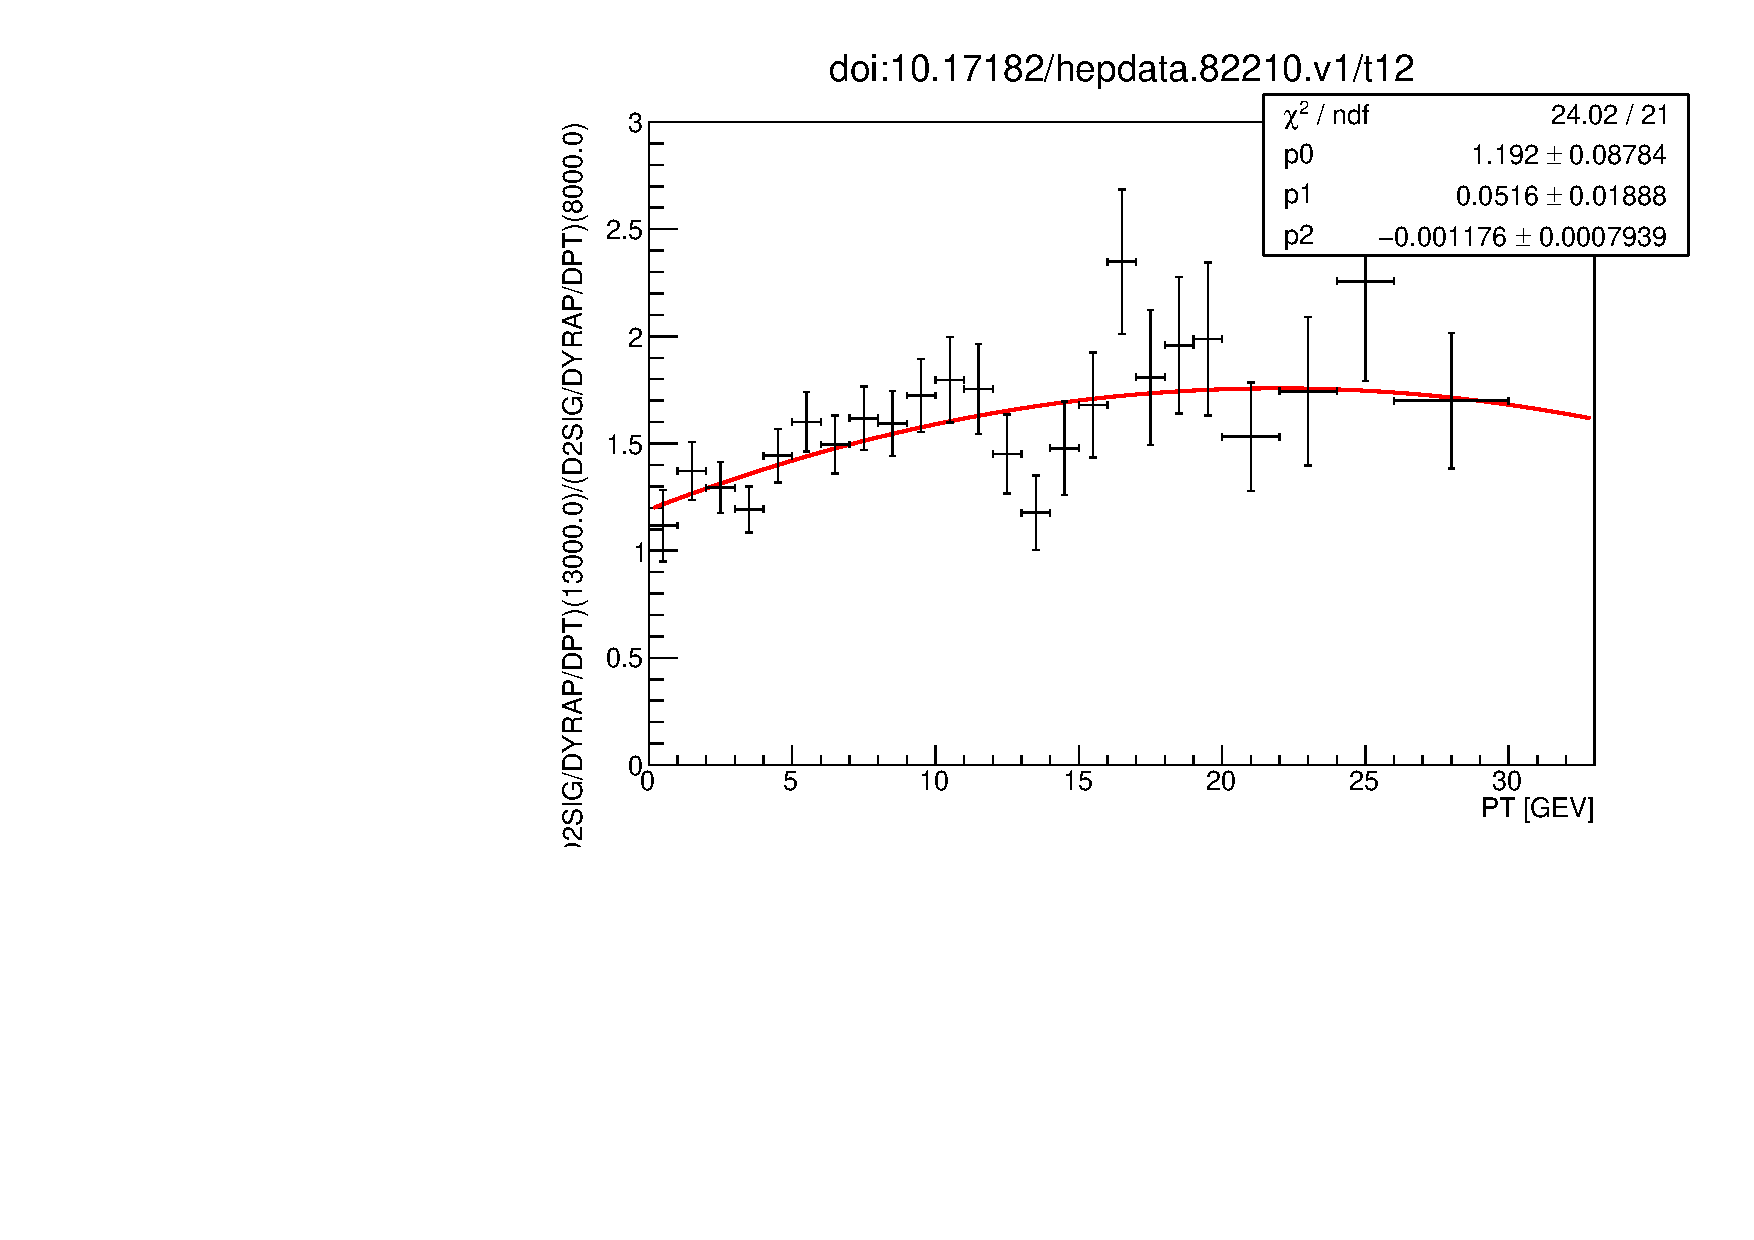
\includegraphics[width=0.32\linewidth]{../oniaDirect/LHCB-13-TeV/ups3s-13to7eta20to25.pdf}
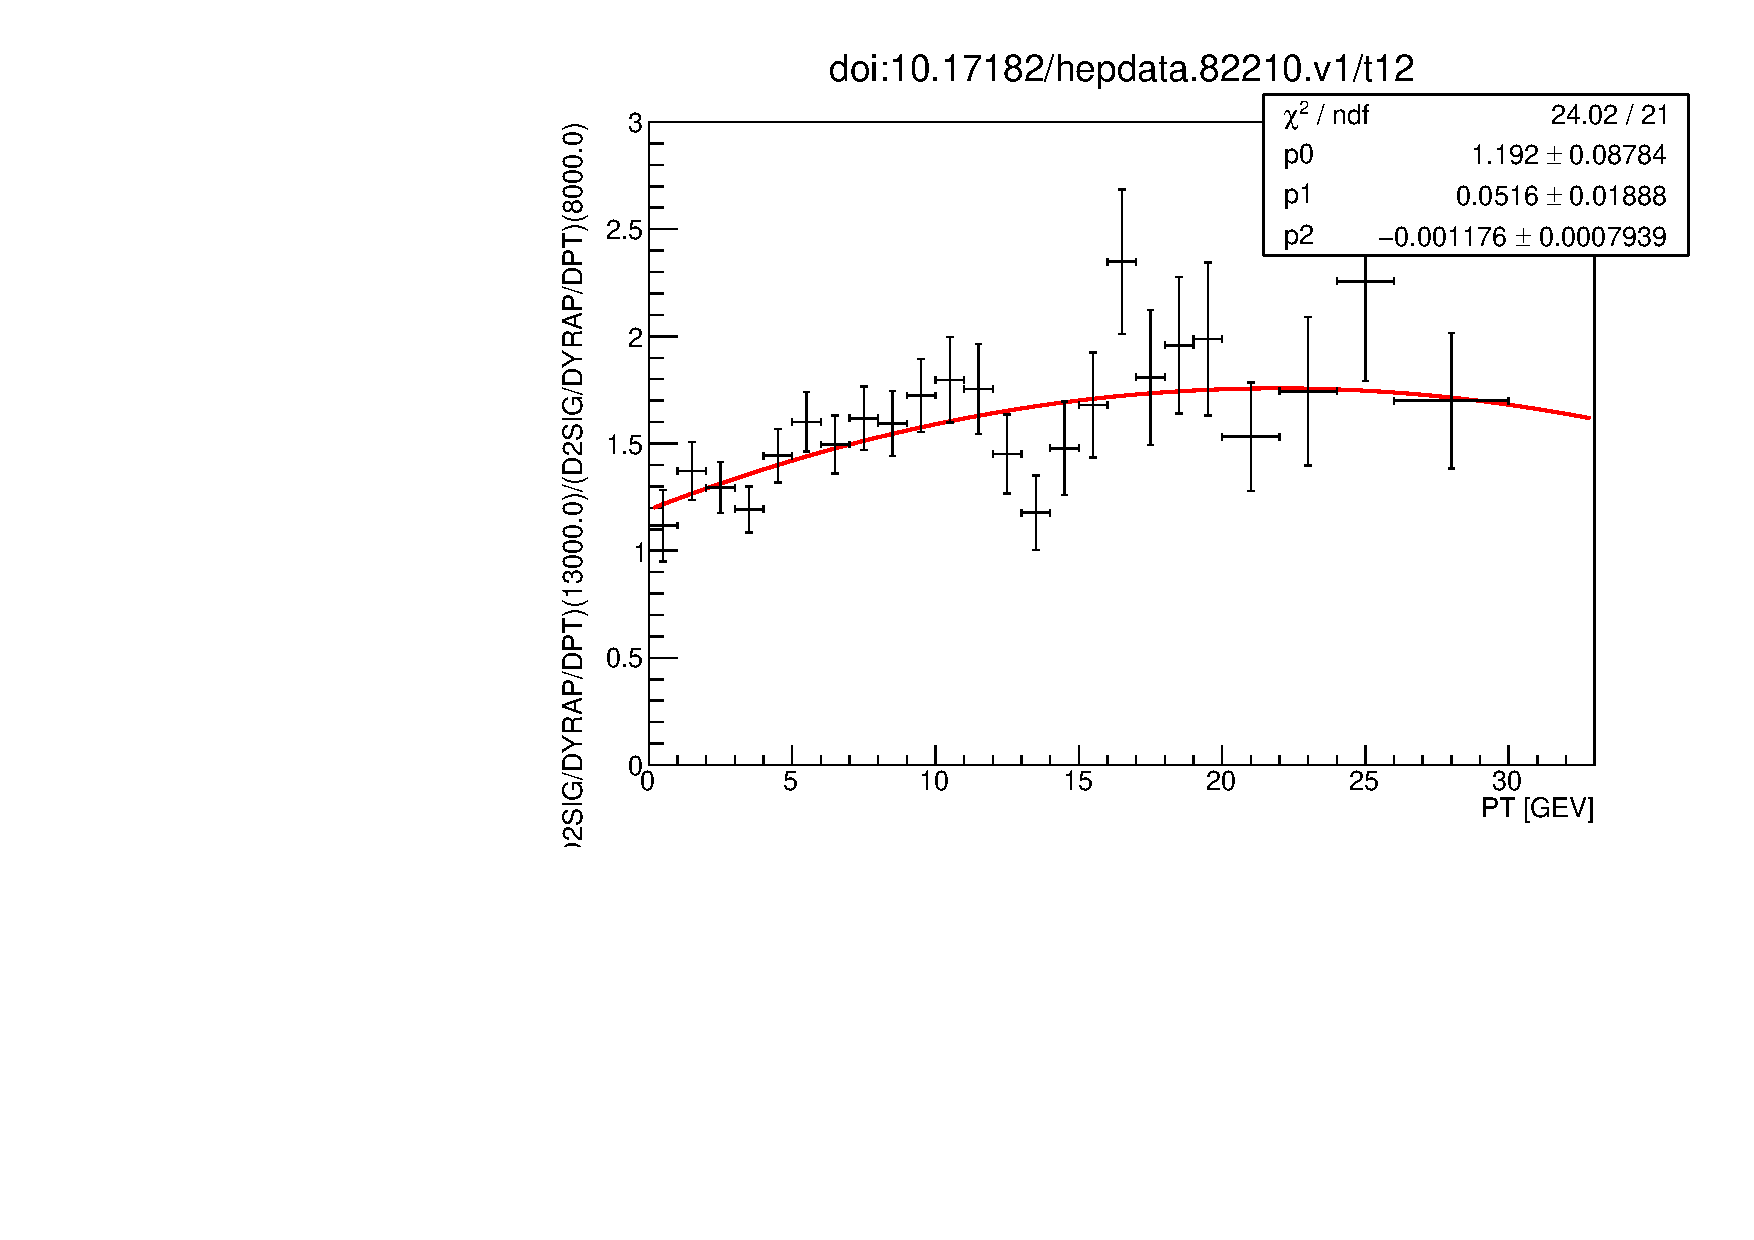
\includegraphics[width=0.32\linewidth]{../oniaDirect/LHCB-13-TeV/ups3s-13to7eta20to25.pdf}
\end{adjustwidth}
\caption{\protect Ratio of 13 to 7 GeV $\Upsilon$ cross-section for $2.0 < y < 2.5$
  from LHCb~\cite{Aaij:2018pfp}.  From left to right: 1S, 2S, 3S. 
  The quadratic fits are ours.}
\label{fig:upsratio}
\end{figure}


  
  As a result we decided to use 7 TeV data for $p_T <$ 20 GeV and the CMS
  13 TeV data at higher $p_T$.  A key ingredient is the ratio of 13 and 7
  GeV $\Upsilon$ production cross-sections.  These have been measured
  for $p_T > 20$ GeV and $|\eta| <$ 1.2 by CMS,
  see Figure 2 of Reference~\cite{Sirunyan:2017qdw}. The ratios
  are about 1.7 at $p_T$ = 20 GeV, irrespective of $\Upsilon$ state
  (1S, 2S, or 3S), and increase slowly to about 2
  at $p_T$ = 40 GeV.  The ratios have also been measured by
  LHCb~\cite{Aaij:2018pfp}
  all the way down to zero $p_T$ for $2.0 < y < 2.5$, see Figure~\ref{fig:upsratio}.
  The LHCb ratios in the 20-30 GeV region measured at slightly higher
  $y$ are in agreement with the more central
  ratios measured by CMS.

\begin{figure}
\begin{adjustwidth}{-2cm}{-2cm}
\centering
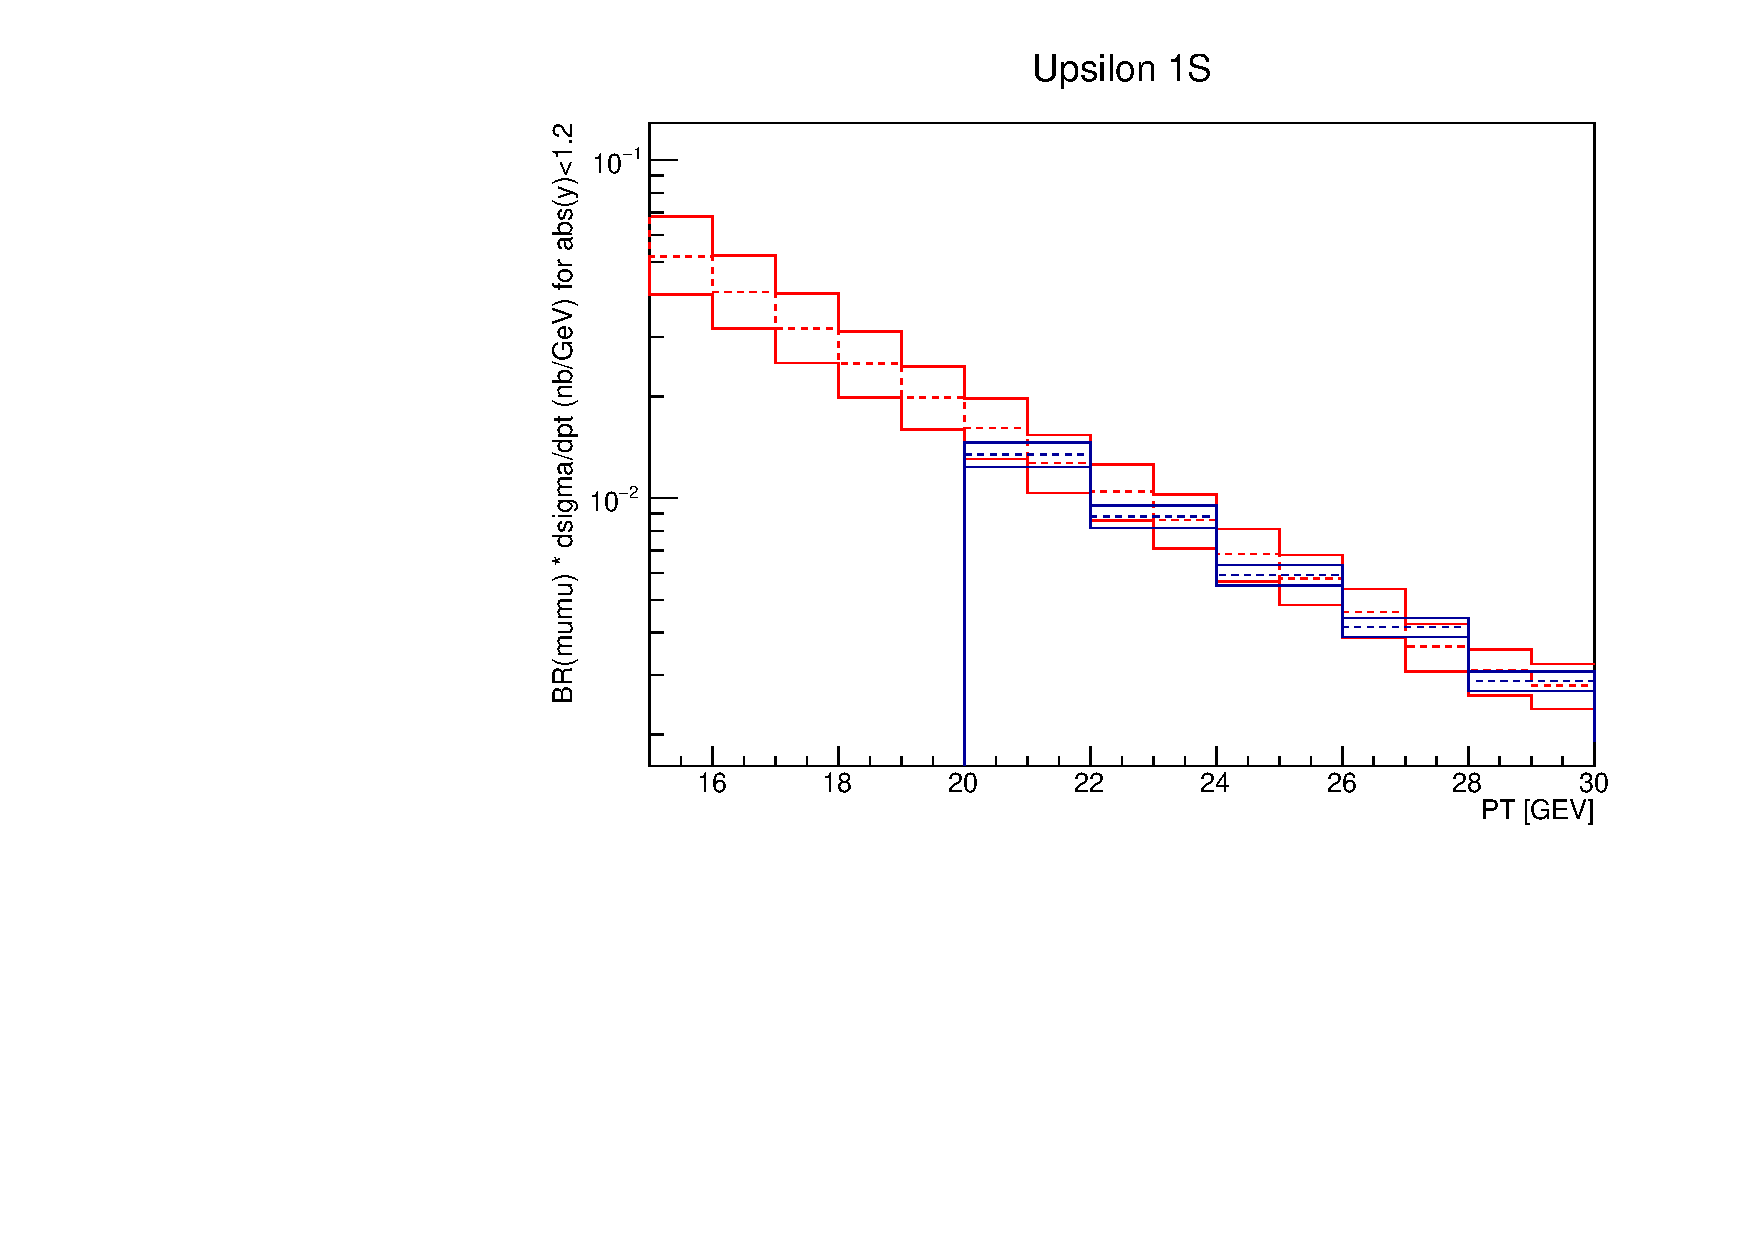
\includegraphics[width=0.32\linewidth]{../oniaDirect/upsilon/upsilon-1s-atlas-cms-comparison.pdf}
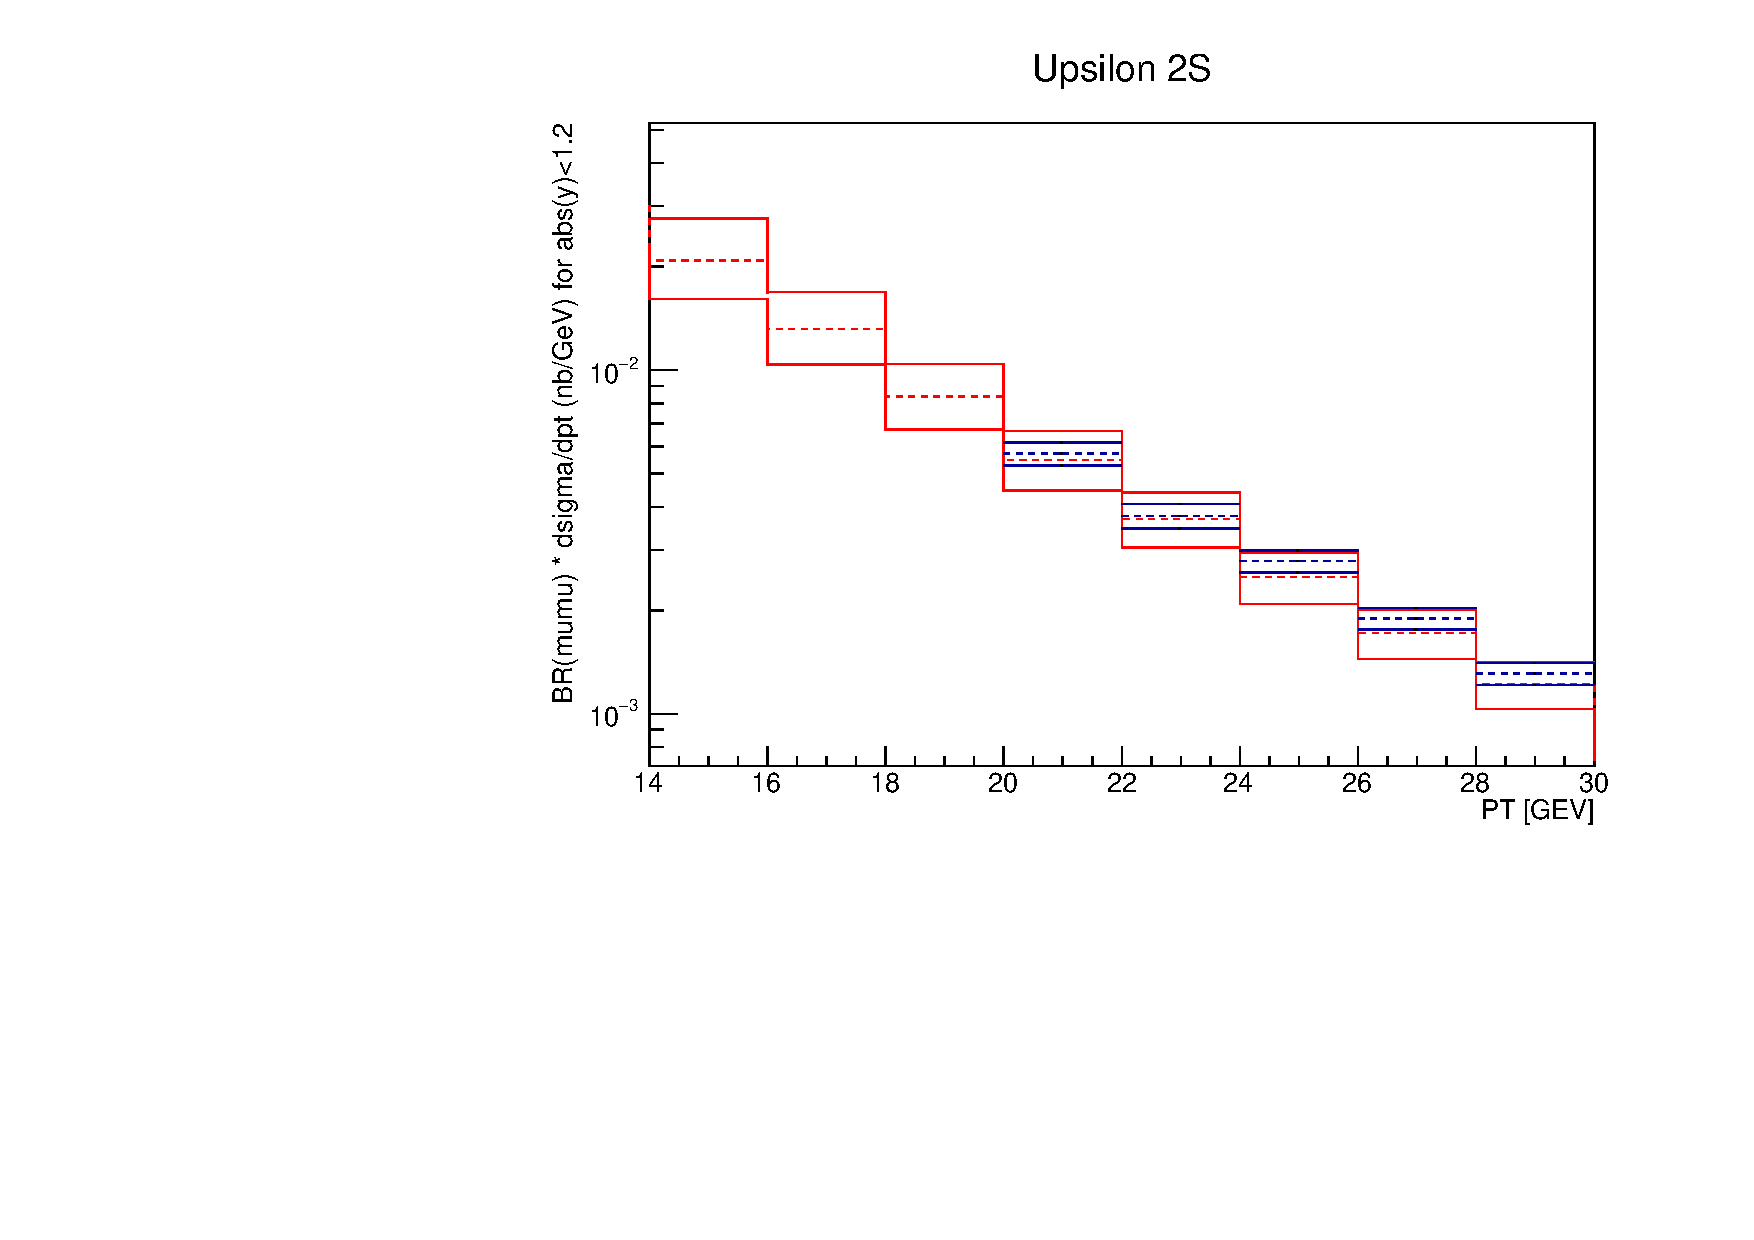
\includegraphics[width=0.32\linewidth]{../oniaDirect/upsilon/upsilon-2s-atlas-cms-comparison.pdf}
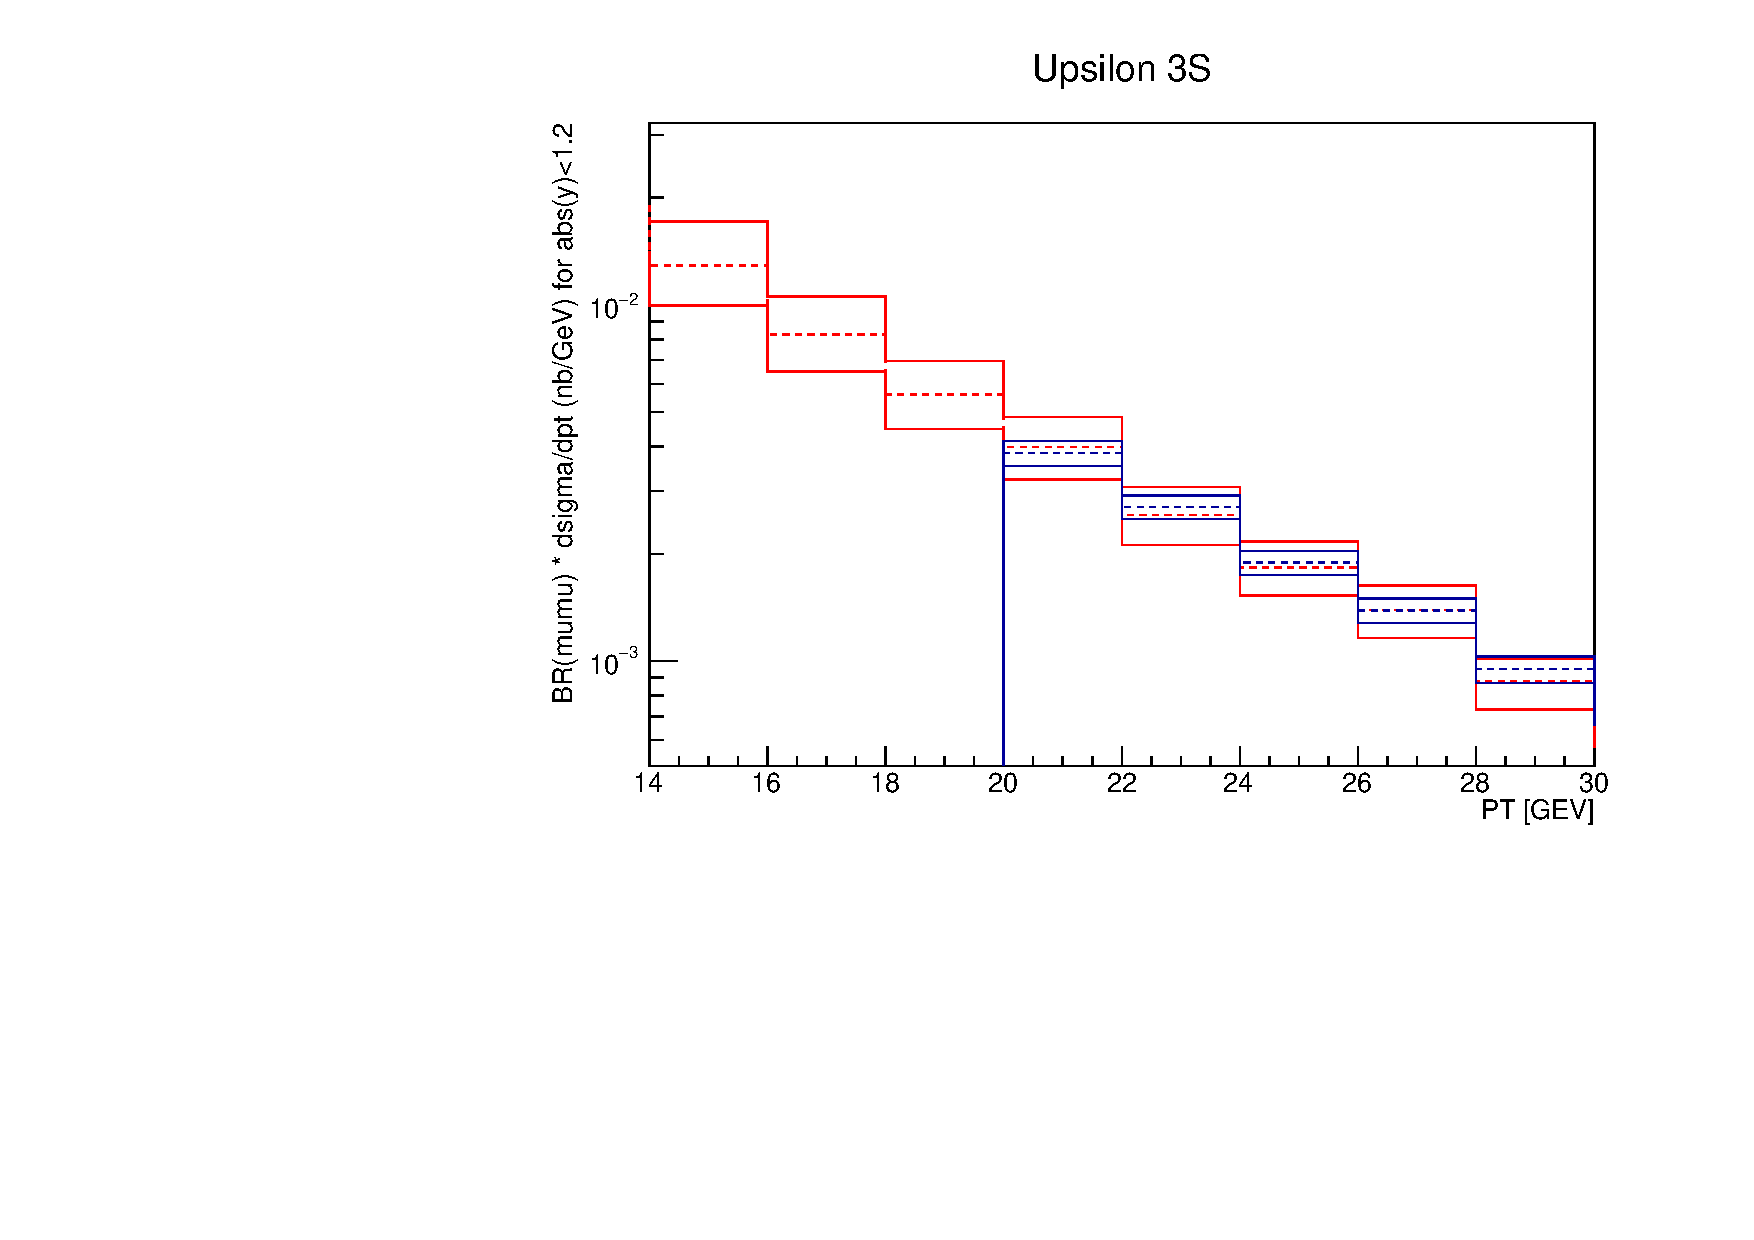
\includegraphics[width=0.32\linewidth]{../oniaDirect/upsilon/upsilon-3s-atlas-cms-comparison.pdf}
\end{adjustwidth}
\caption{\protect Comparison of the rescaled 7 GeV Atlas $\Upsilon$ spectra (red) with the
  13 GeV CMS spectra (blue) in the neighborhood of 20 GeV, where the matching of
  the two spectra takes place.  From left to right: 1S, 2S, 3S.
  The dashed lines represent the central values, the solid
  lines cover the uncertainty range.  This is ${\cal B}(\Upsilon \to \mu\mu) \cdot
  \rm{d}\sigma/\rm{d}p_T$ in nb/GeV integrated
  over $|\eta| <$ 1.2.}
\label{fig:checkMatch}
\end{figure}

\begin{figure}
\begin{adjustwidth}{-2cm}{-2cm}
\centering
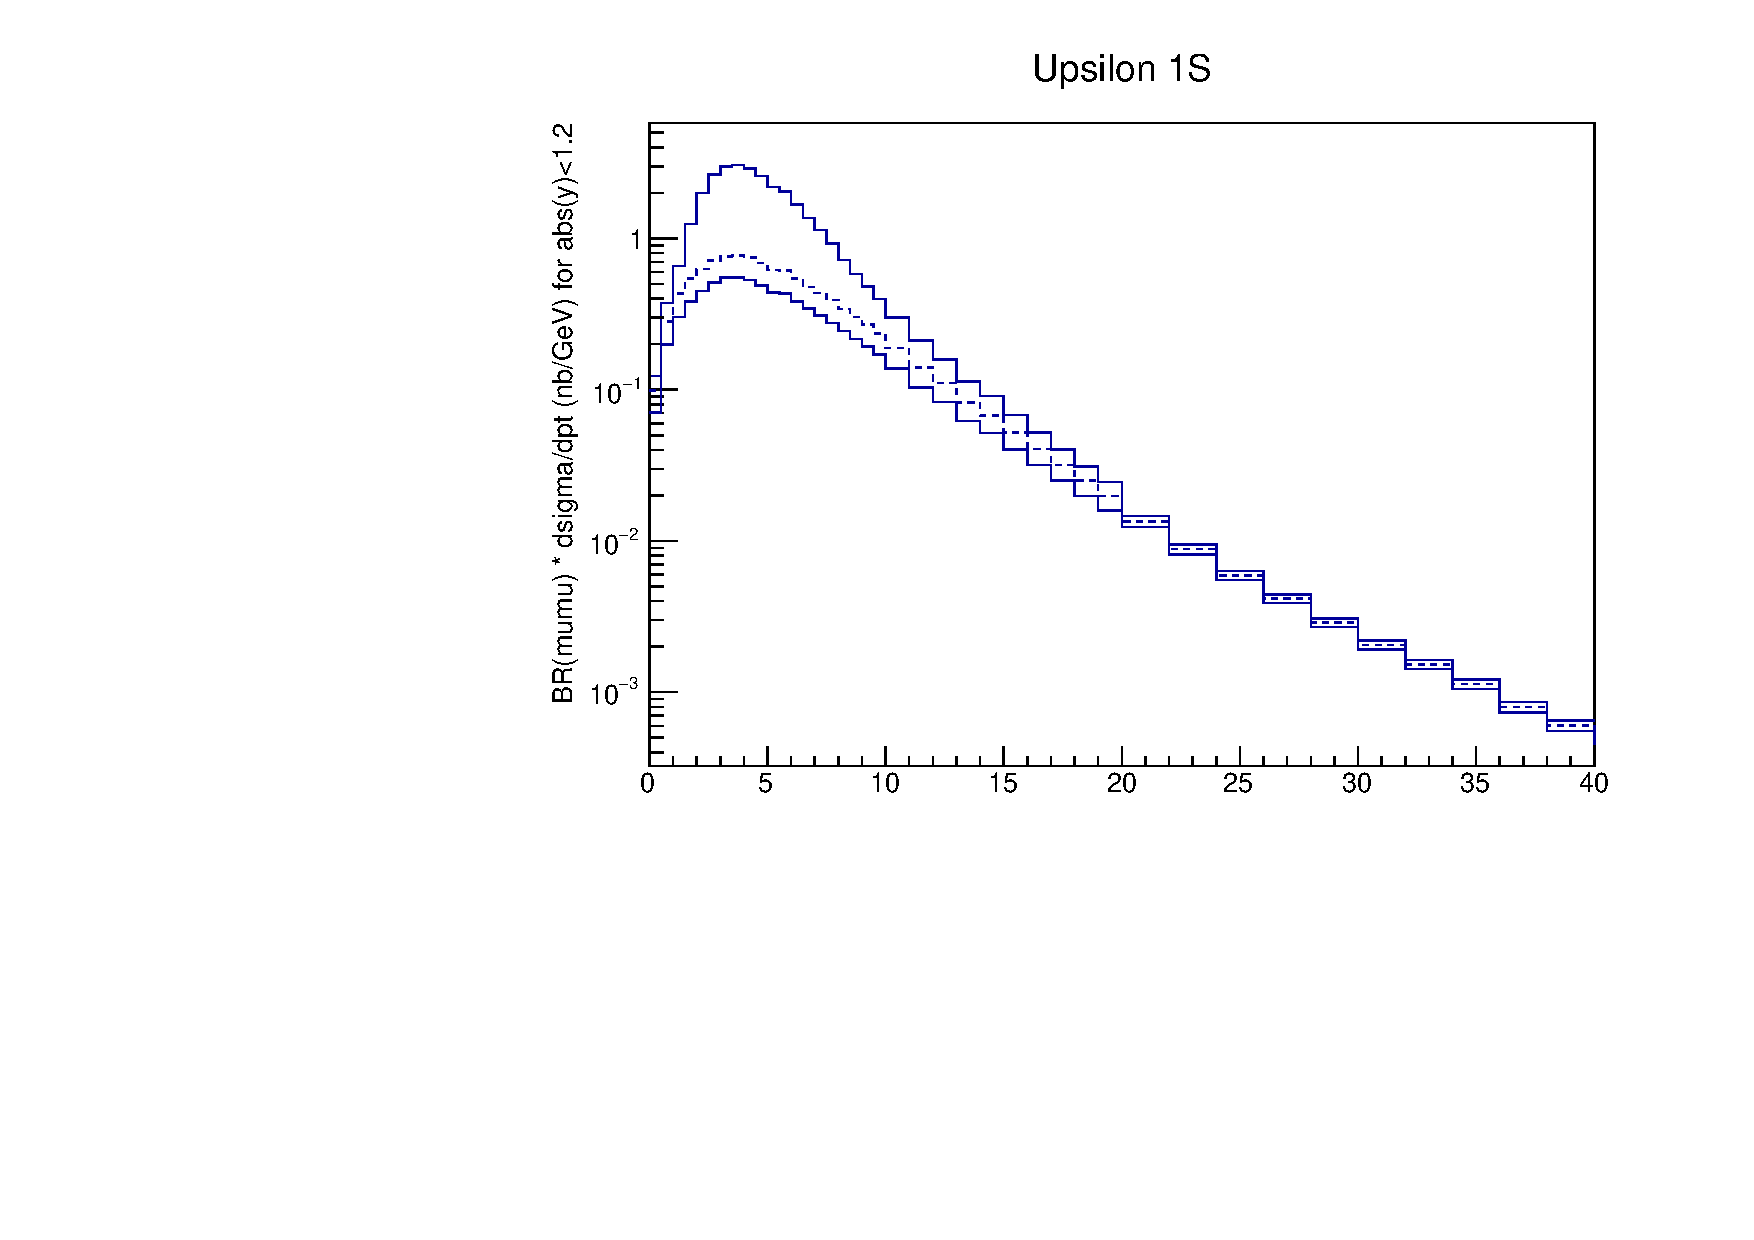
\includegraphics[width=0.32\linewidth]{../oniaDirect/upsilon/ups1s-full.pdf}
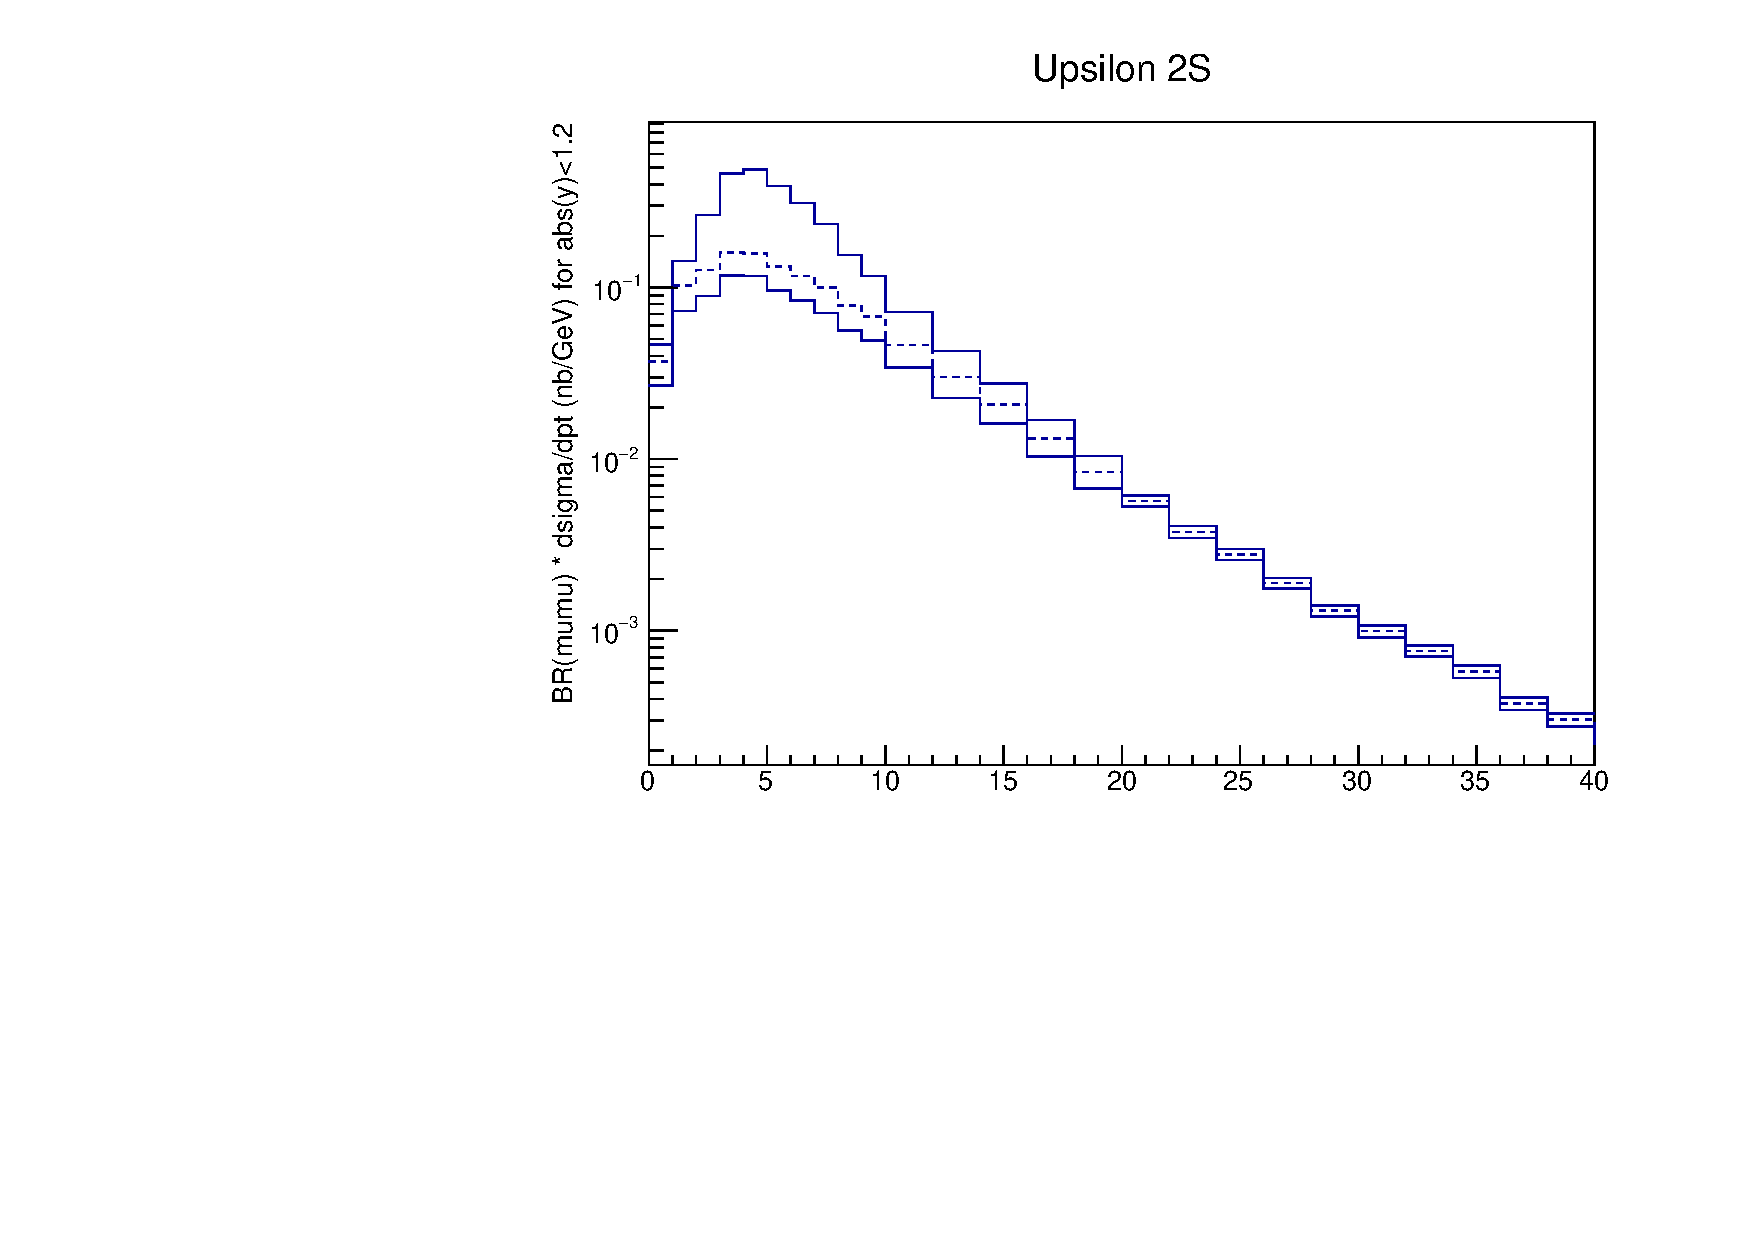
\includegraphics[width=0.32\linewidth]{../oniaDirect/upsilon/ups2s-full.pdf}
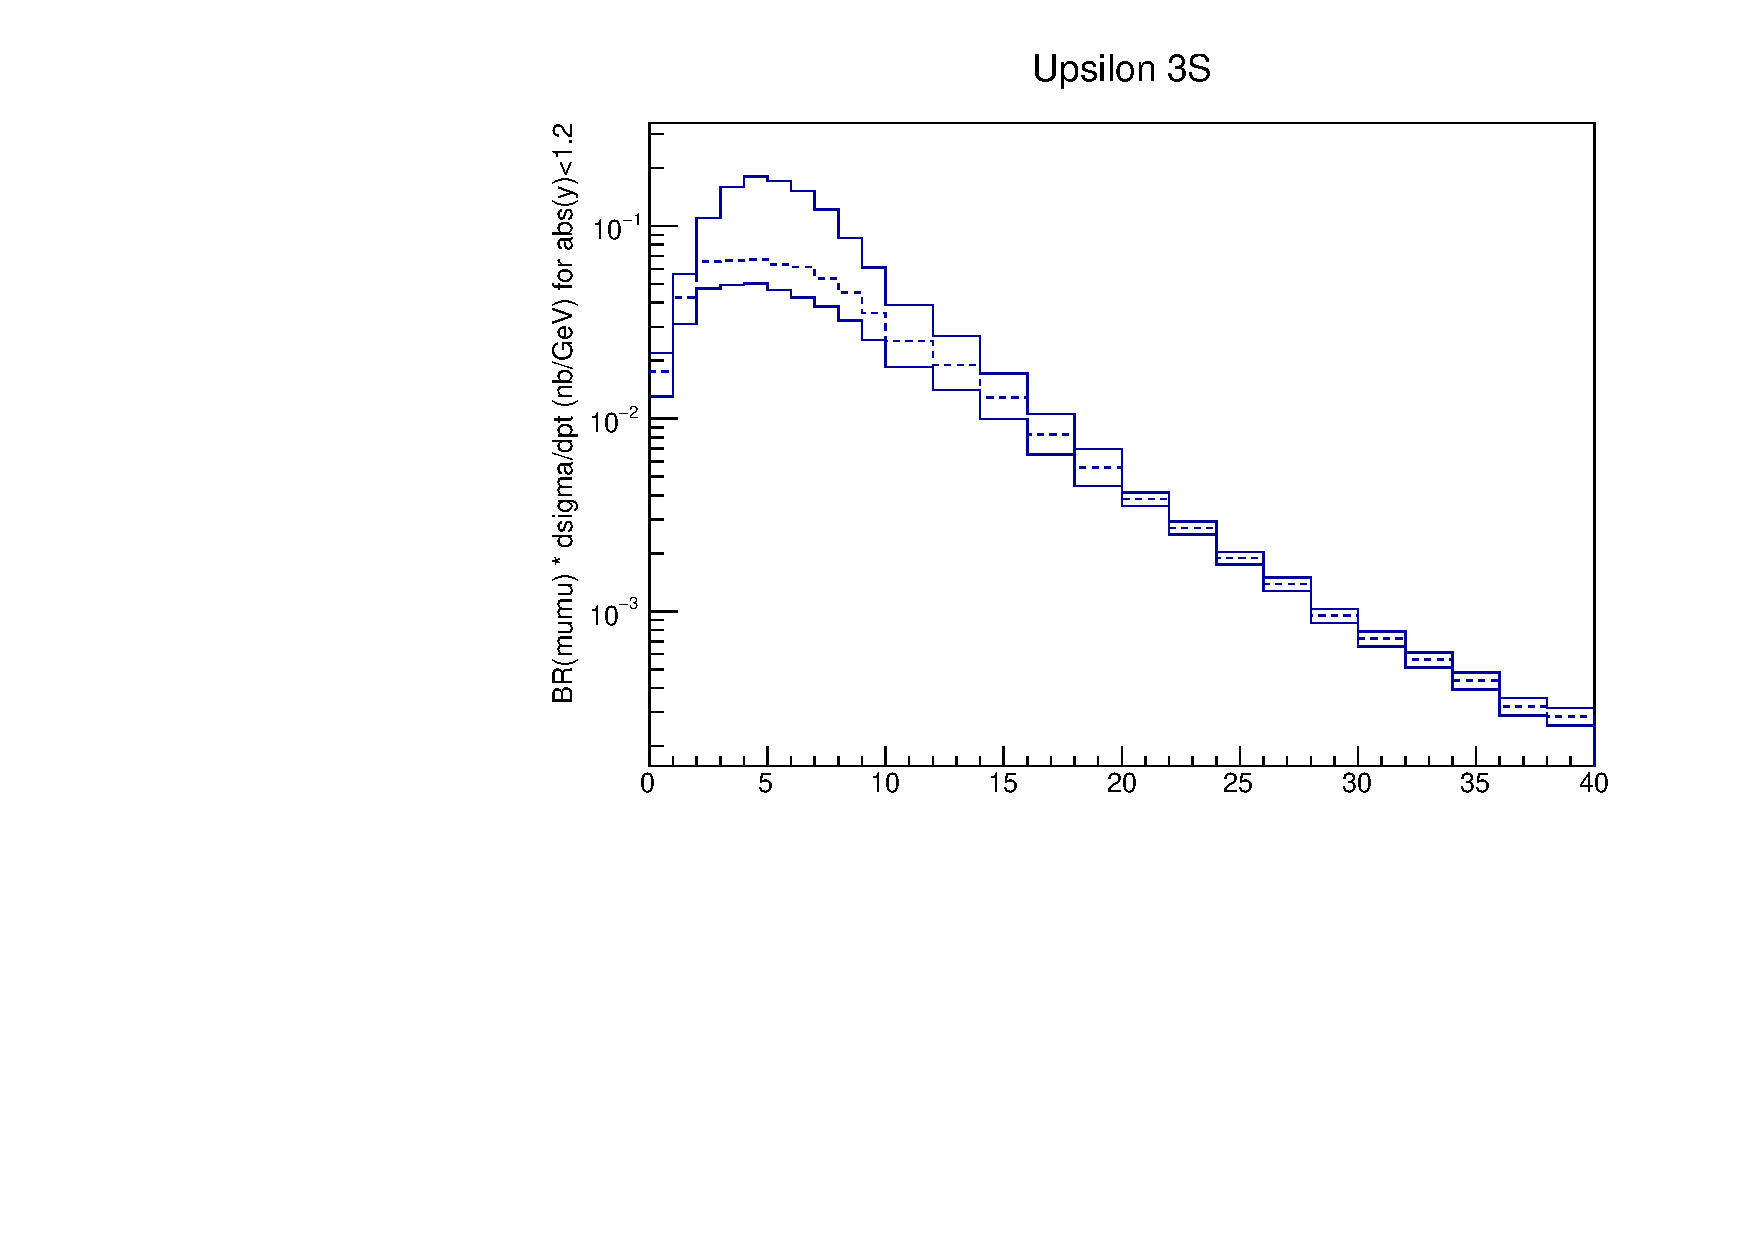
\includegraphics[width=0.32\linewidth]{../oniaDirect/upsilon/ups3s-full.pdf}
\end{adjustwidth}
\caption{\protect Combined Atlas 7 TeV, CMS 13 TeV $\Upsilon$ spectra.
  From left to right: 1S, 2S, 3S. 
The dashed line represent the central value, the solid
  lines cover the uncertainty range.  This is ${\cal B}(\Upsilon \to \mu\mu) \cdot
  \rm{d}\sigma/\rm{d}p_T$ in nb/GeV integrated
  over $|\eta| <$ 1.2.}
\label{fig:upsFinal}
\end{figure}

  
Consequently,  we rescale the {\bf measured} 7 GeV {\bf central} low
$p_T$ $\Upsilon$ spectra to 13 TeV using the curves of
Figure~\ref{fig:upsratio};  we combine these with the {\bf measured} 13 TeV 
  {\bf central} high $p_T$ spectra to obtain an inclusive 13 TeV spectra.  The 7 TeV data
  is from Atlas~\cite{Aad:2012dlq}, since it happens to be in a more
  convenient format than the equivalent CMS data.
On the other hand the 13 TeV spectra are from
  CMS~\cite{Sirunyan:2017qdw}, since there is no Atlas measurement at
  13 TeV.

We demonstrate in Figure~\ref{fig:checkMatch} that the
  matching of the Atlas and CMS cross-sections works well.  The combined
  spectra to be used in the event generation are in Figure~\ref{fig:upsFinal}.


\subsubsection{Direct charmonium}
\label{sec:psidirect}
We take the charmonium spectra from theory~\cite{Ma:2010yw, Ma:2010jj, Ma:2014mri}
see Figure~\ref{fig:ma}.  

\begin{figure}
% 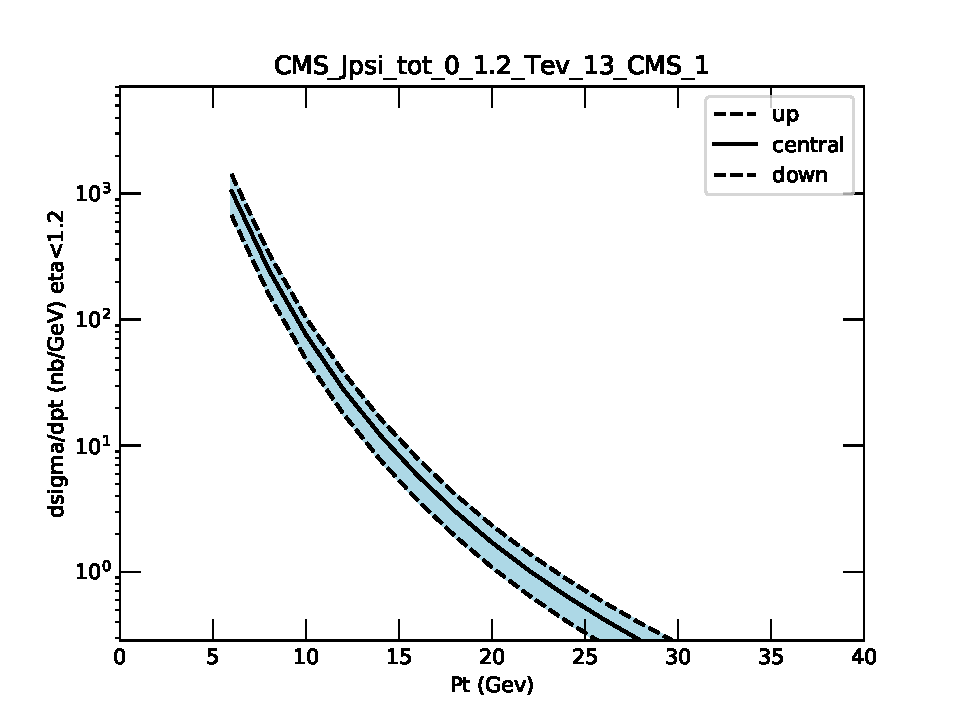
\includegraphics[width=0.48\linewidth]{../oniaDirect/CMS-13-TeV/theory/CMS-Jpsi-tot-0-12-Tev-13-CMS-1.pdf}  
% 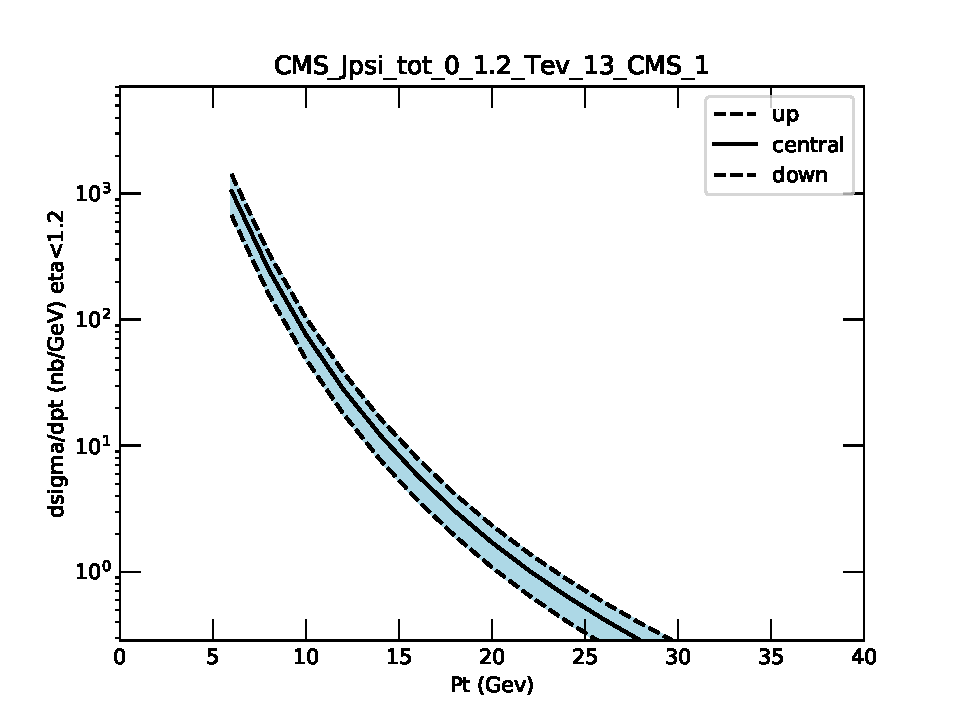
\includegraphics[width=0.48\linewidth]{../oniaDirect/CMS-13-TeV/theory/CMS-Jpsi-tot-0-12-Tev-13-CMS-1.pdf}
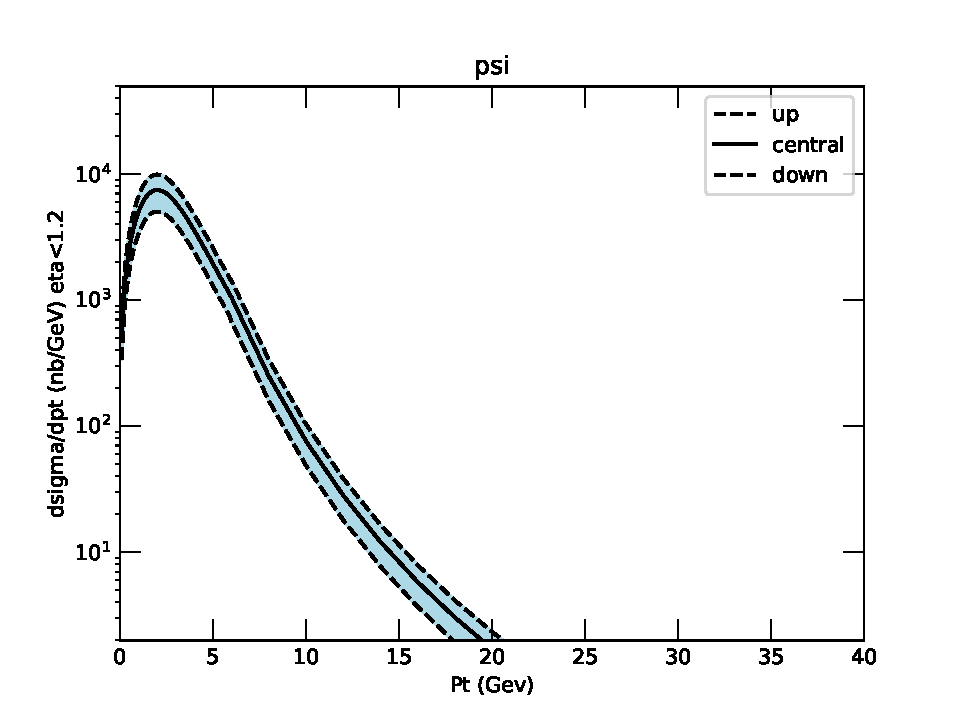
\includegraphics[width=0.48\linewidth]{../oniaDirect/CMS-13-TeV/theory/psiLowPt/psiDirect_fullRange.pdf}  
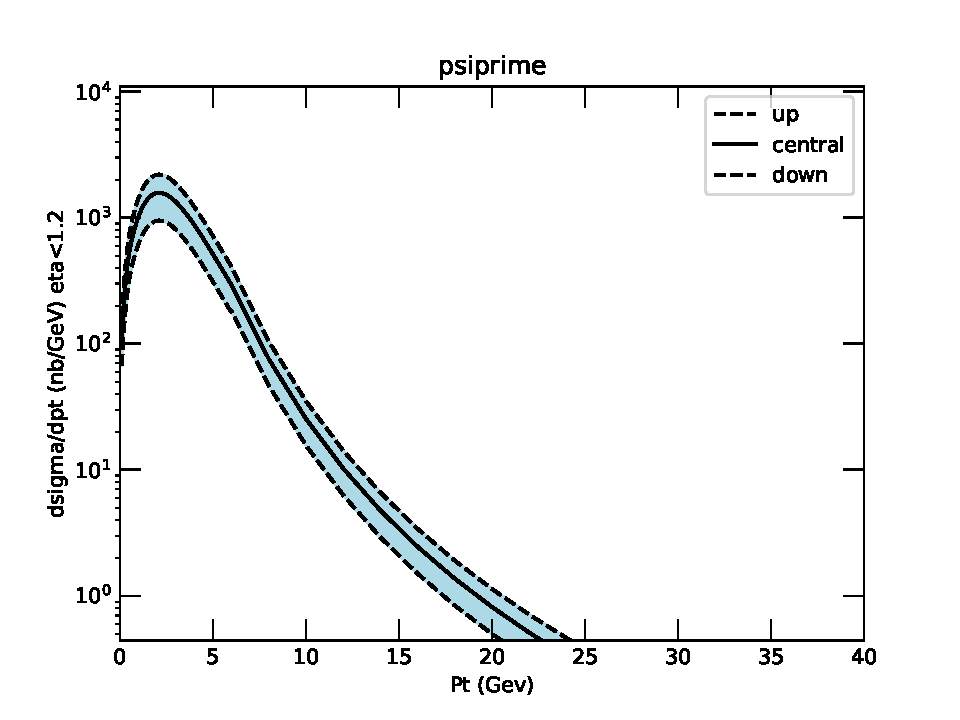
\includegraphics[width=0.48\linewidth]{../oniaDirect/CMS-13-TeV/theory/psiLowPt/psiprimeDirect_fullRange.pdf}  
  \caption{Transverse momentum distributions of J/$\psi$ (left) 
and $\psi'$ from direct production. The units are nb/GeV and the 
distributions 
are integrated over $|\eta|<1.2$.}
  \label{fig:ma}
\end{figure}


\subsection{J/$\psi$ sanity check}

Most of the J/$\psi$ cross-section is from direct production, see
Figure~\ref{fig:sanity}, left.  As a sanity check we also show
the fractions of J/$\psi$ and $\psi'$ from b decays measured
at lower energy, see 
Figure~\ref{fig:sanity}, right\cite{Khachatryan:2010yr}.

\begin{figure}
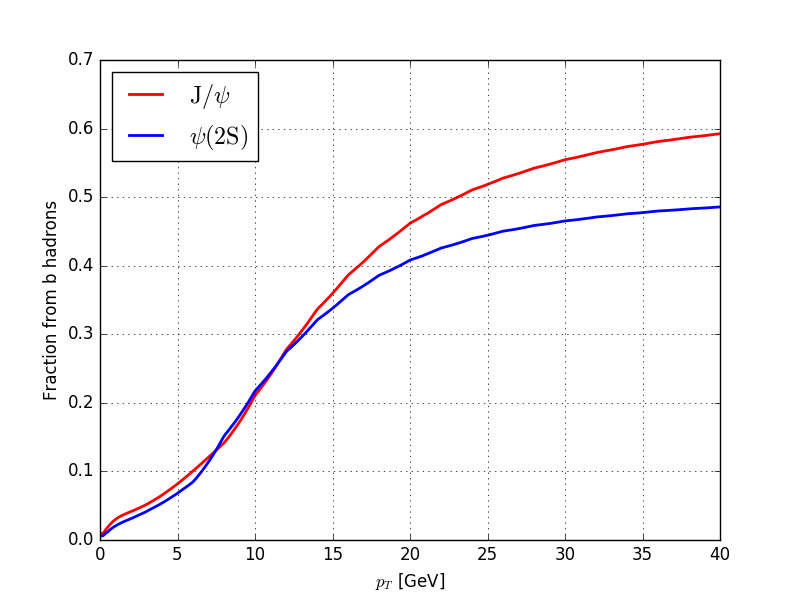
\includegraphics[width=0.53\linewidth]{plots/fraction-from-b-theory.png}
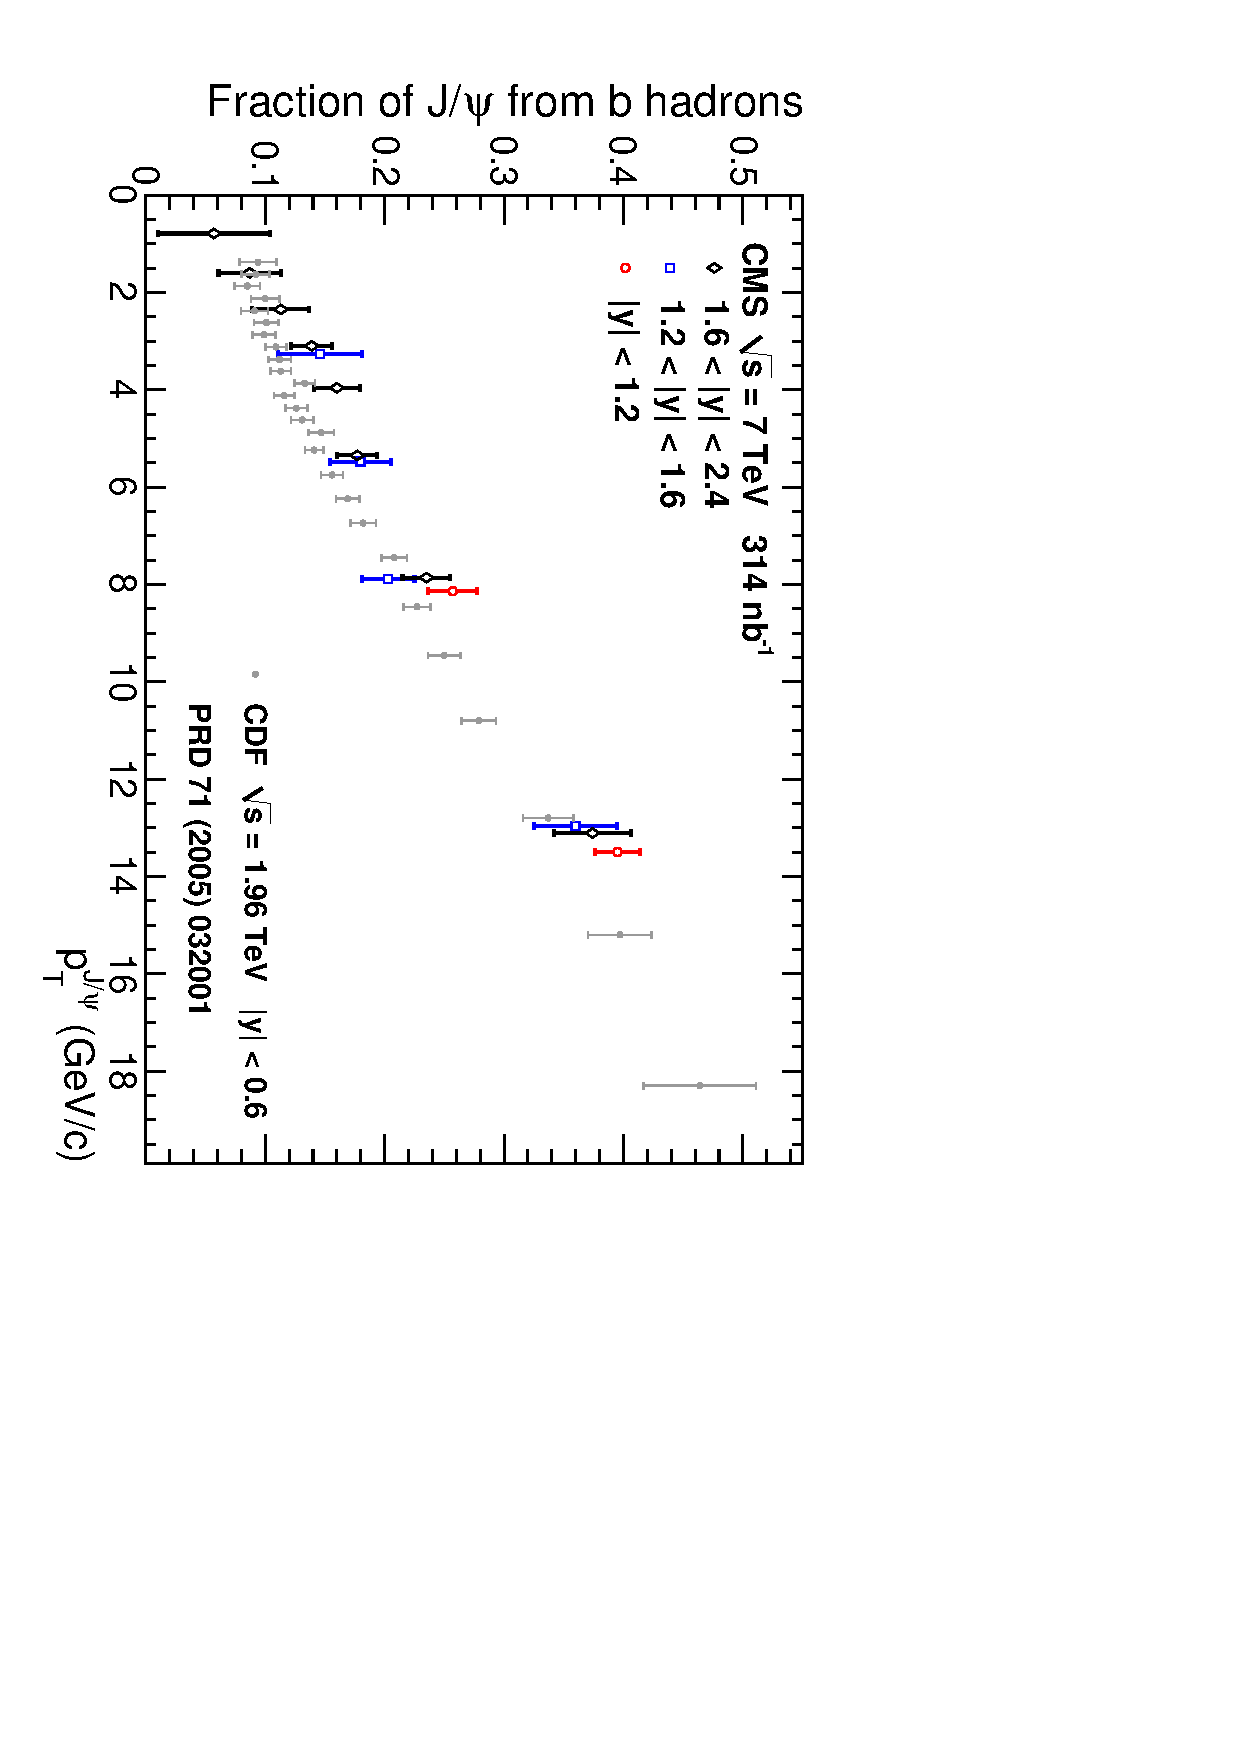
\includegraphics[height=0.46\linewidth, angle=90]{plots/bFraction-CMS-314nb-CDF.pdf}
\caption{Fraction of charmonium from b decays according to the calculations used in
  this note (left), and the corresponding measurement (J/$\psi$ only) at lower energy (right).
 The left plot is for $|\eta|<1.2$.}
  \label{fig:sanity}
\end{figure}



\subsection{$\pi^0$, $\eta$, $\eta'$, $\phi$, $\rho$, and $\omega$}
\label{sec:mesons}

We generate these from Pythia.  The measurement of the 
$\pi^{\pm}$
$p_T$ spectrum from CMS\cite{Sirunyan:2017zmn} is in good agreement
with Pythia 8 Minimum Bias at low momentum.  This gives us some
confidence in Pythia Min Bias, and consequently we use this MC for all
mesons.  We do not attempt to use QCD $2 \to 2$ at very low $p_T$ since the 
process is infrared divergent.

Pythia {\tt SoftQcd:nonDiffractive} includes all
hard QCD processes\cite{wwwPythia} so in principle this is all that is
needed.    However, we run out of statistics at high $p_T$.  So 
at high $p_T$ we stitch together the Min Bias distributions with 
distributions obtained from QCD $2 \to 2$ at moderate $p_T$.

%% Eventually we will generate Pythia events in ``standalone'' mode to
%% be independent of CMS software.  For now we use existing CMS Monte
%% Carlos for MinBias and for QCD.  

This has been done both with CMS MC samples and with events generated
from standalone Pythia, using the same public CUETP8M1 tune (\cite{CMS:tunes}, table 3).
They have been verified to give equivalent results.

The QCD samples are
``$p_T$-binned'', using the \texttt{PhaseSpace:pTHat[Min/Max]} parameters in Pythia, 
in bins 15-30 GeV, 30-50 GeV, and 50-80 GeV.  
The MinBias cross-section is taken to be 69.8 mb (CMS-recommended value).  
Then the stitching procedure is the following:
\begin{itemize}
\item The QCD samples are first normalized to their LO cross-sections.
\item Next, we estimate a ``QCD-MinBias scale factor'' by integrating
  over some $p_T$ region where the MinBias/QCD ratio is roughly flat.
\item The QCD samples are all renormalized by this scale factor.
\item The samples are stitched together by visually picking the 
$p_T$ where the curves cross each other.
\end{itemize}
\noindent The resulting $p_T$ curves are shown in
Figure~\ref{fig:mesons}.  It is not clear what kind of uncertainties
we should assign.  Eventually we'll have to come up with something (50\%?).


\begin{figure}
  \centering
  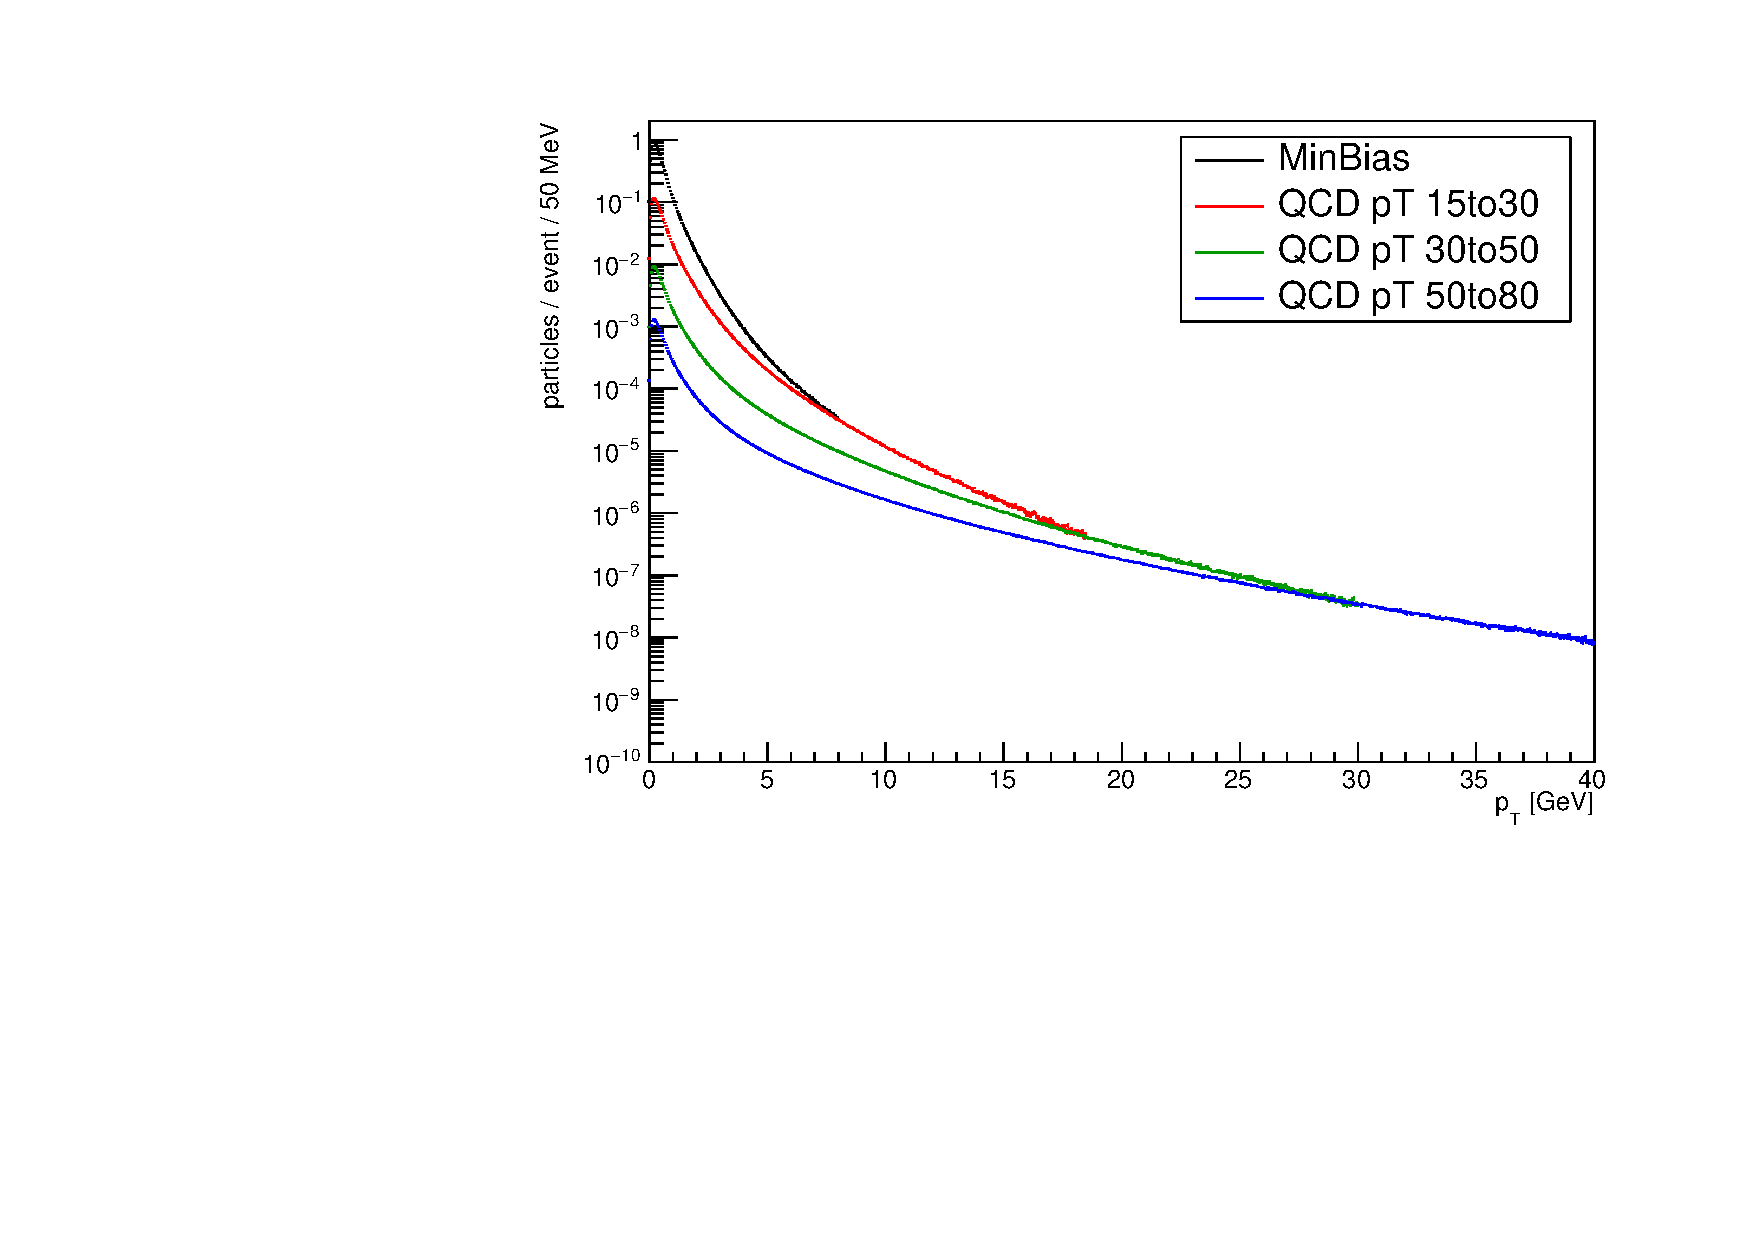
\includegraphics[width=0.48\linewidth]{plots/h_pi0.pdf}
  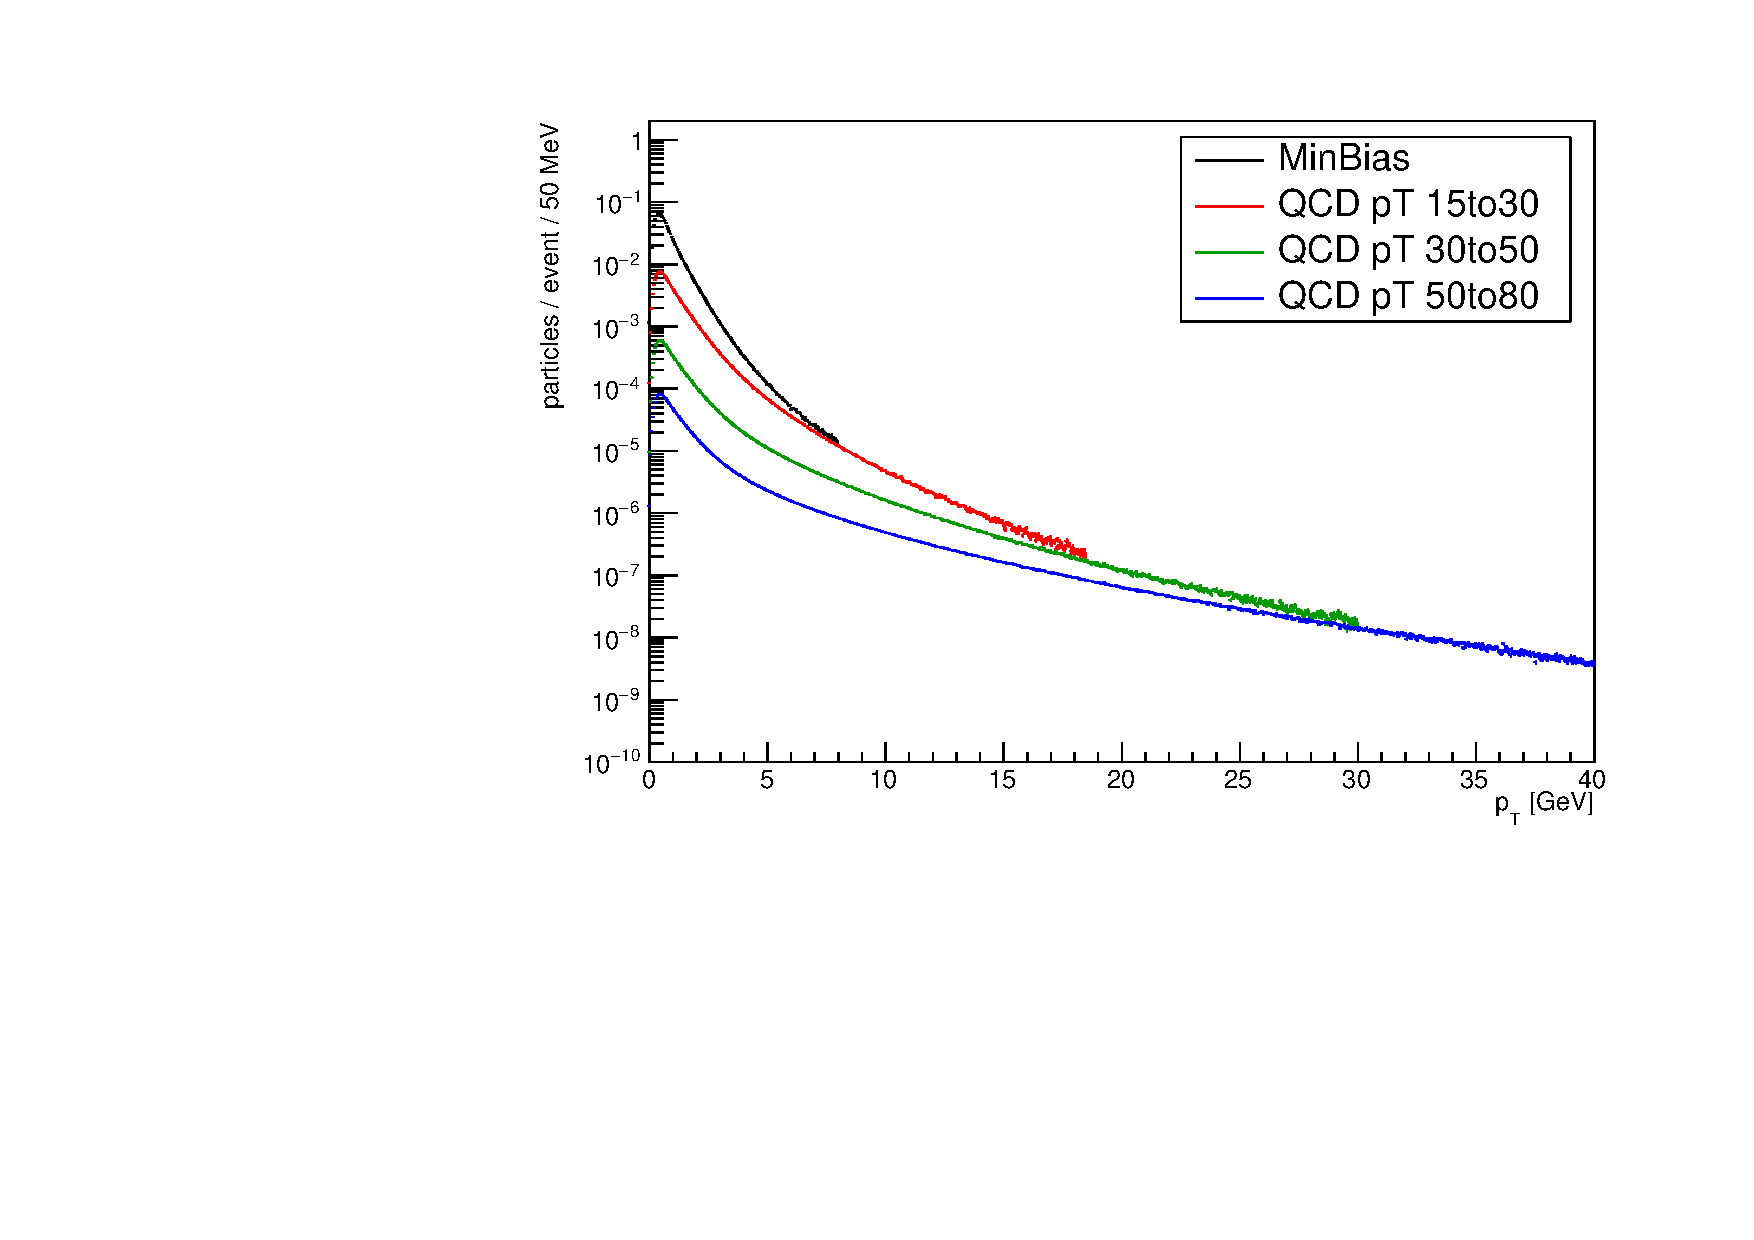
\includegraphics[width=0.48\linewidth]{plots/h_eta.pdf} \\
  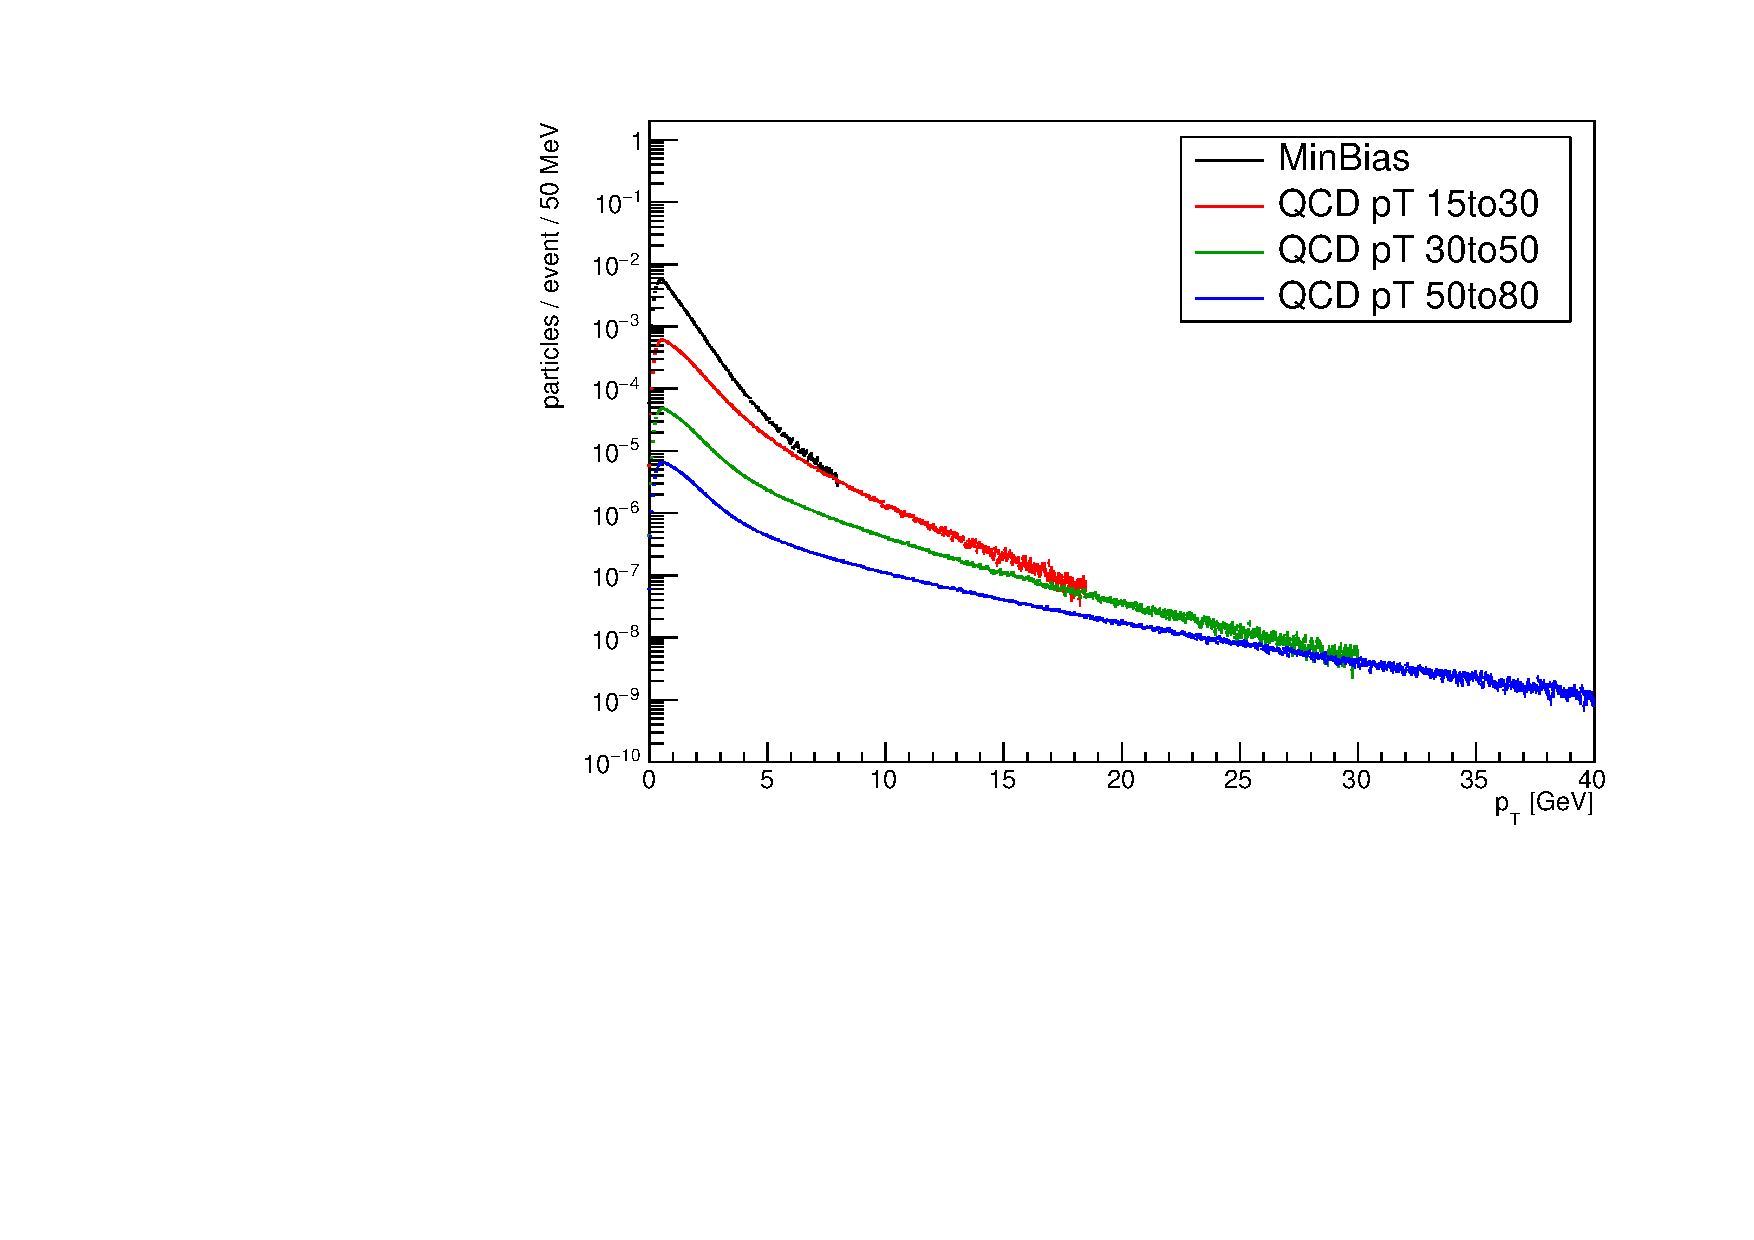
\includegraphics[width=0.48\linewidth]{plots/h_etap.pdf}
  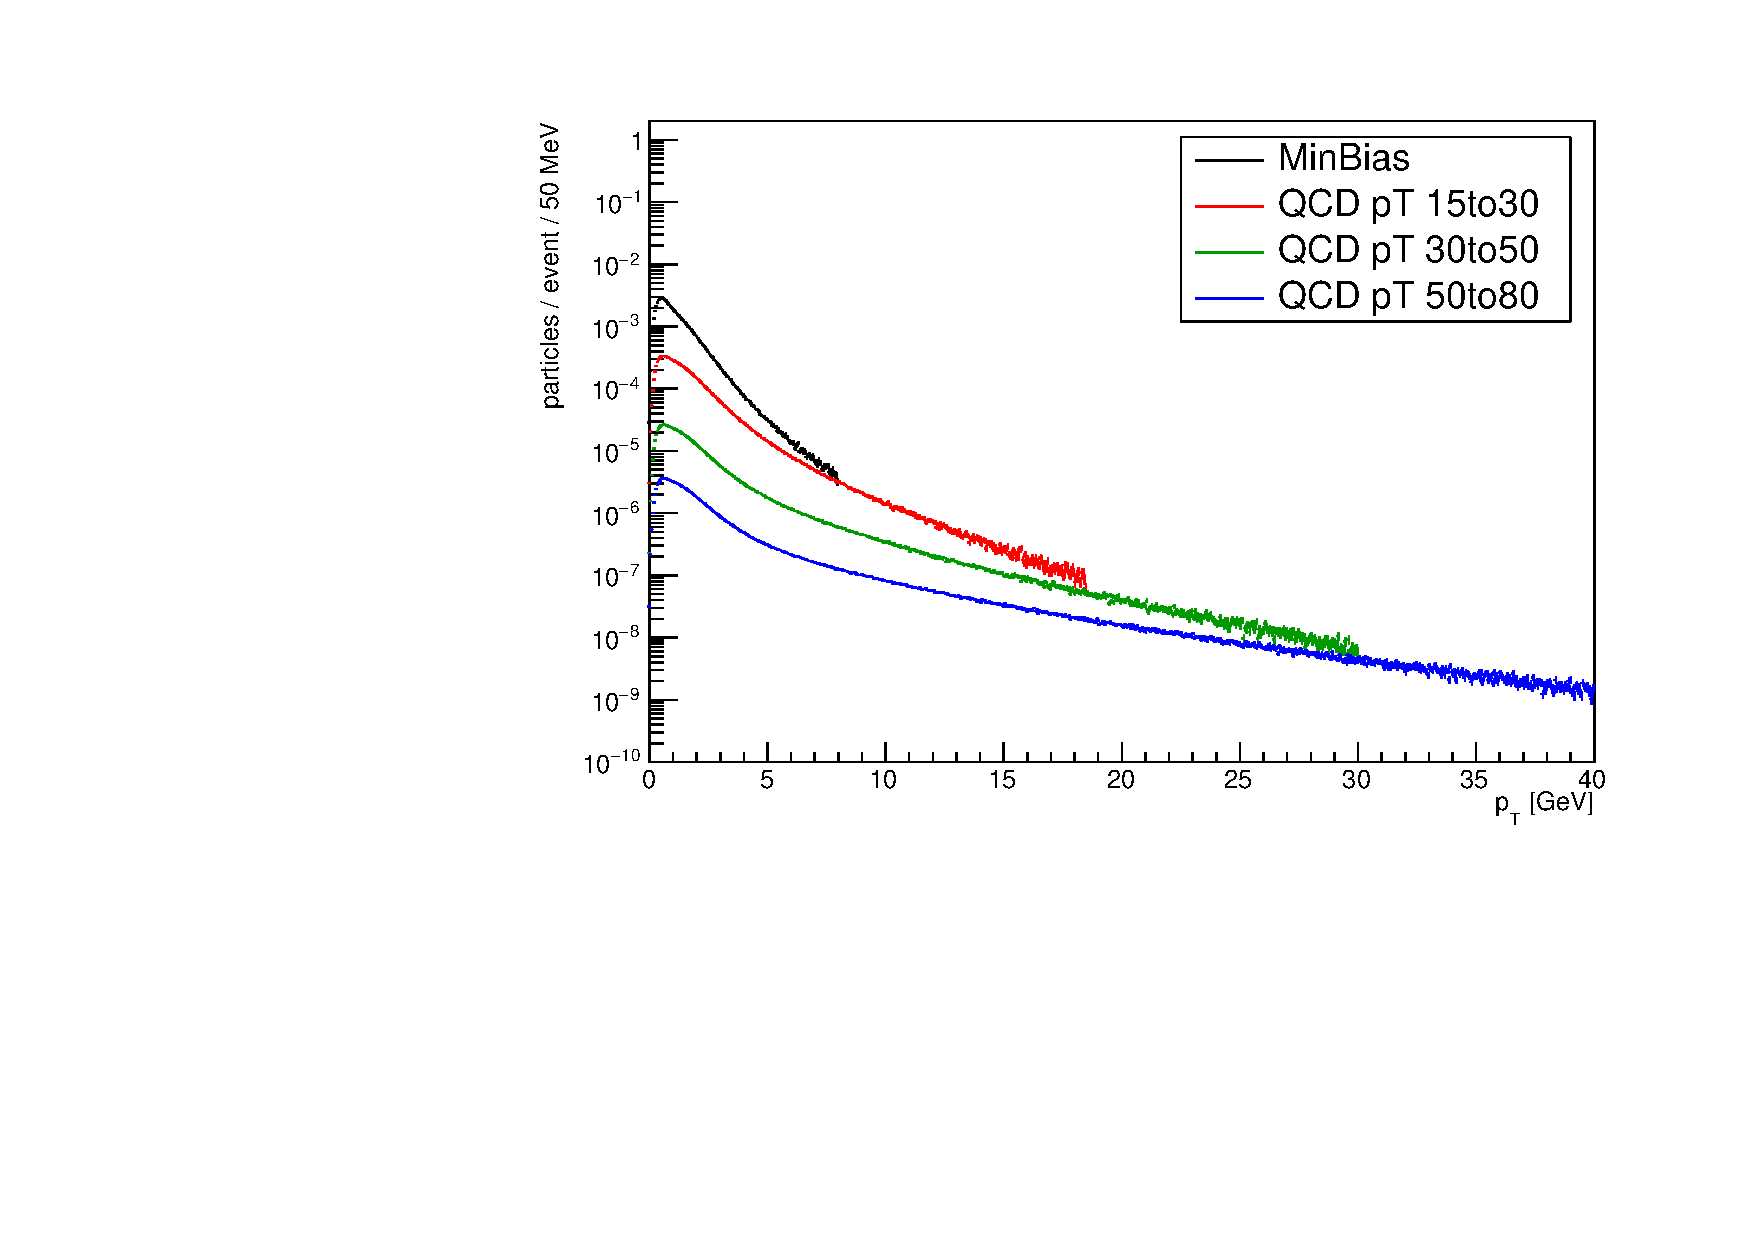
\includegraphics[width=0.48\linewidth]{plots/h_phi.pdf} \\
  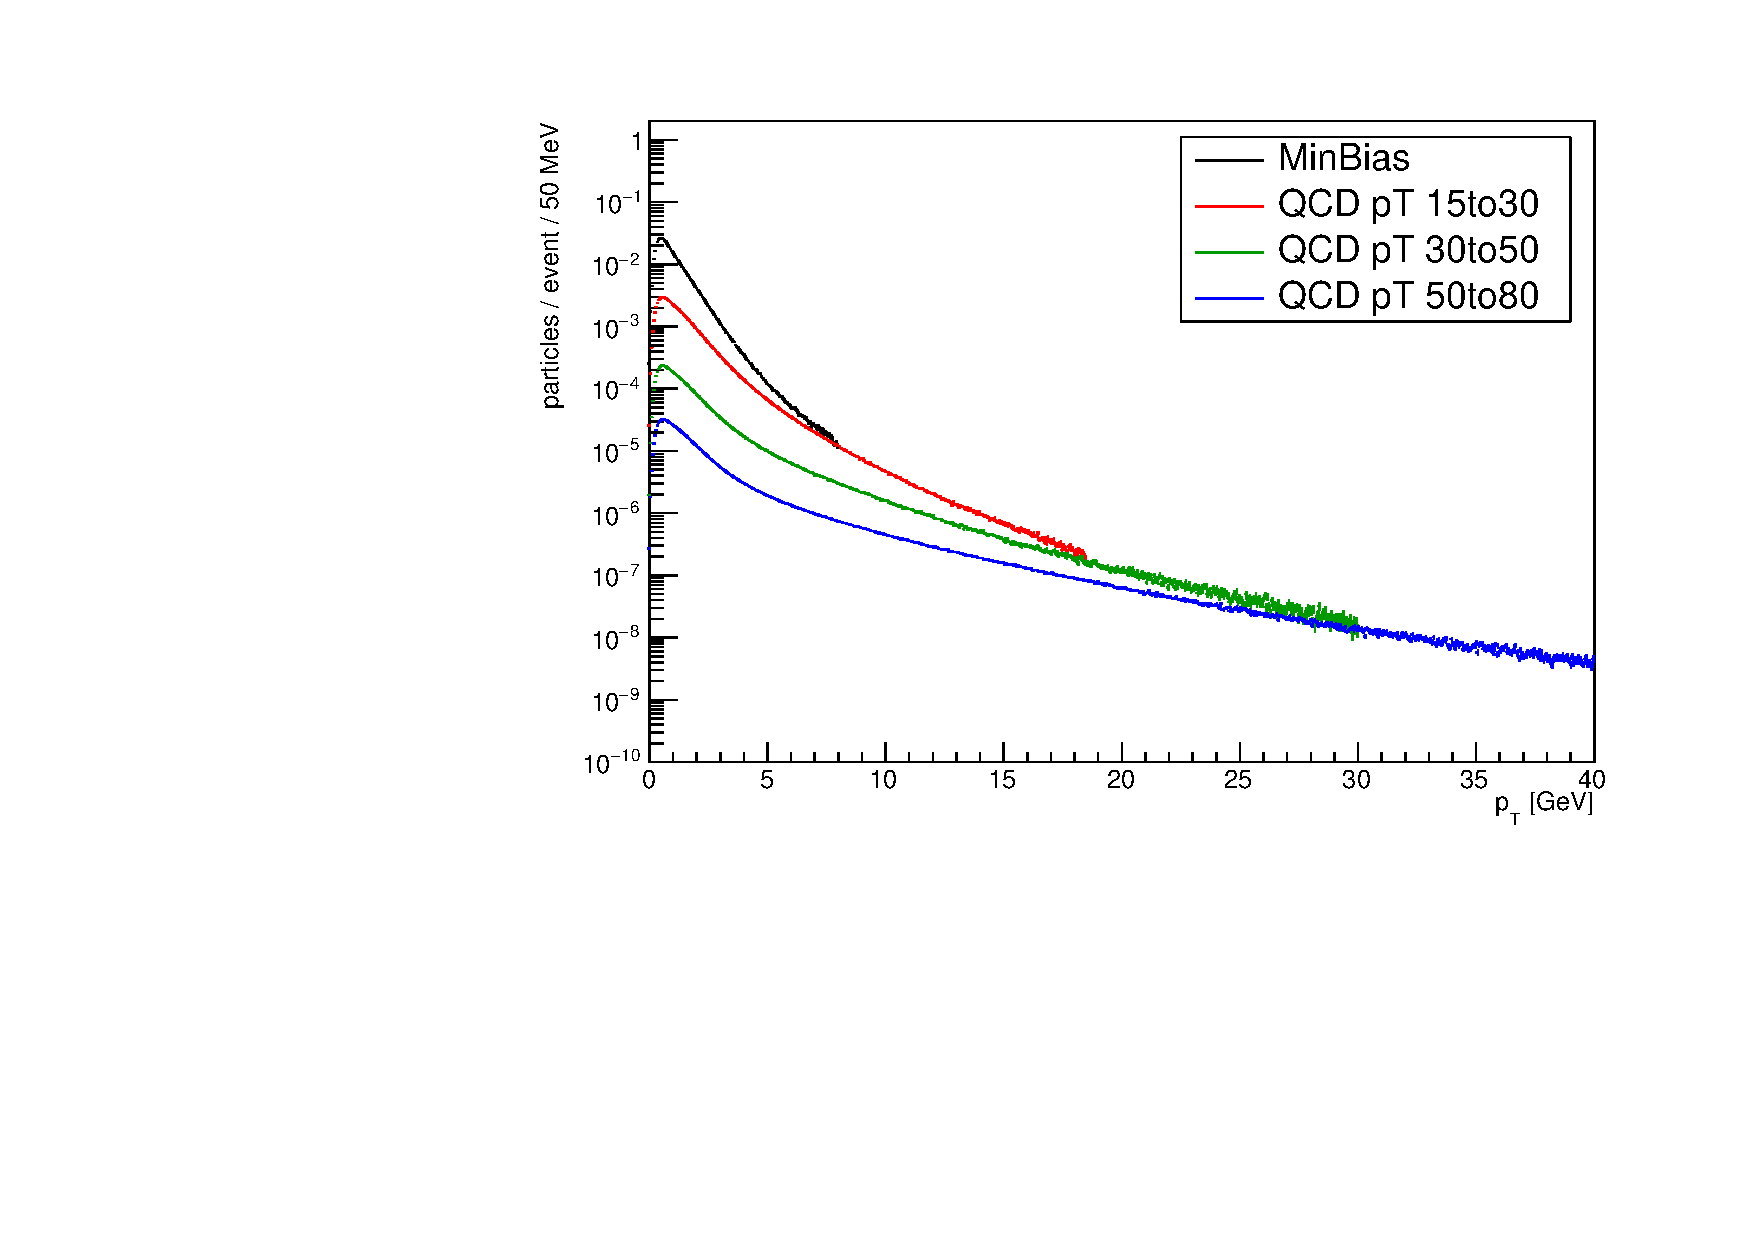
\includegraphics[width=0.48\linewidth]{plots/h_rho.pdf}
  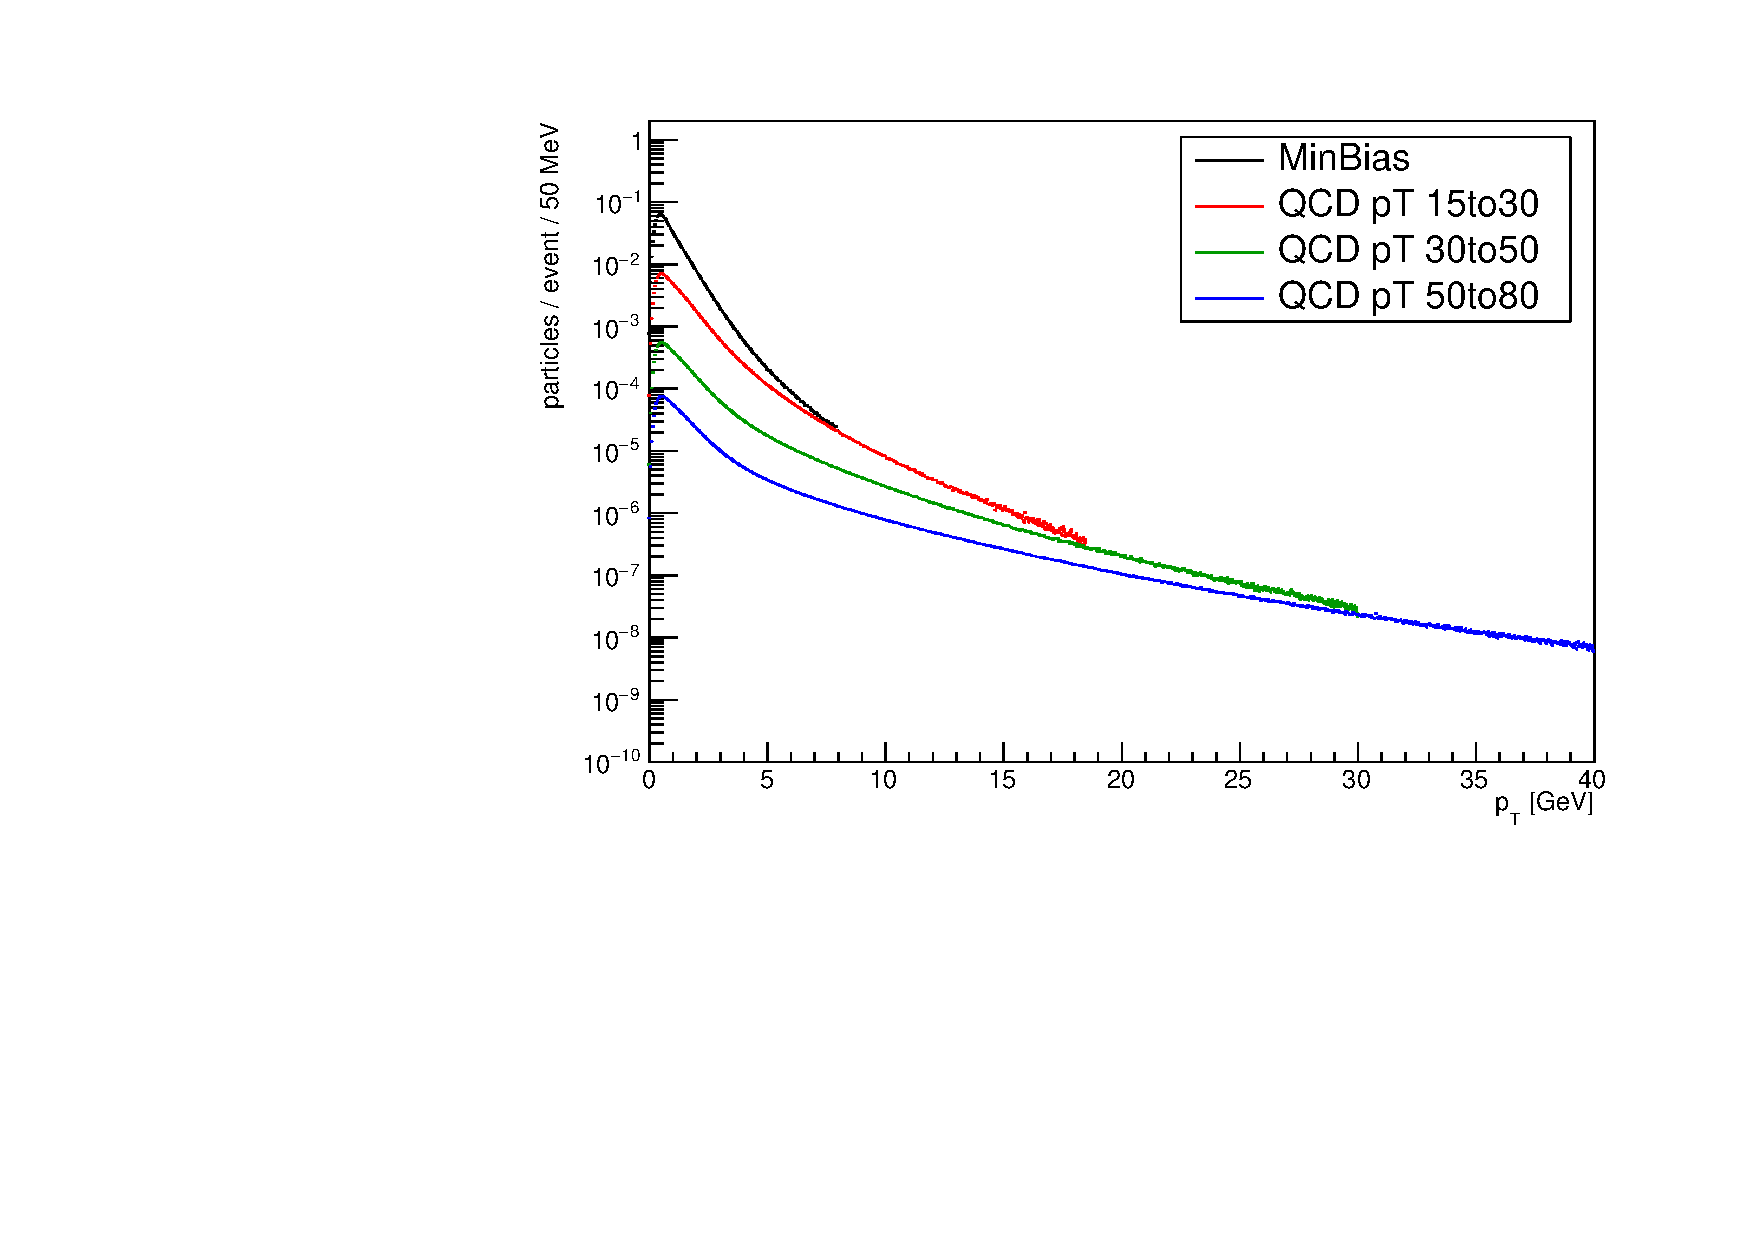
\includegraphics[width=0.48\linewidth]{plots/h_omega.pdf} \\
  \caption{\protect Transverse momentum distributions of 
$\pi^0$, $\eta$, $\eta'$, $\phi$, $\rho$, and $\omega$, top left
to bottom right, for $|\eta| < 1$.}
\label{fig:mesons}
\end{figure}

\clearpage


\section{Putting cross sections and BR together}
\label{sec:bottom-line}

The total cross section for milliCharged particle production (excluding
DY) is shown in Fig.~\ref{fig:total-rates}.  
% Note that the considered contributions from $\eta'$ are negligible. 
As mentioned in
Section~\ref{sec:list}, we are skipping $\eta' \to \pi^+ \pi^- \zeta^+
\zeta^-$.
Note that the other contributions from $\eta'$ in the plot are neglogible.
Since for $\zeta = e$ the branching ratio of the skipped process is four
times higher than
that of $\eta' \to e^+ e^- \gamma$ (Dalitz decay), one worries that
this
process could actually be important.  However, for reasonable $\zeta$
masses, say above 100 MeV, this process is suppressed by phase space
with respect to Dalitz decay, e.g., from the PDG,
BR($\eta' \to \mu^+ \mu^- \gamma$) $\approx$ 1e-4 while
BR($\eta' \to \pi^+ \pi^- \mu^+ \mu^-$) $<$ 3e-5.  So we can safely ignore it.


\begin{figure}
  \begin{center}
  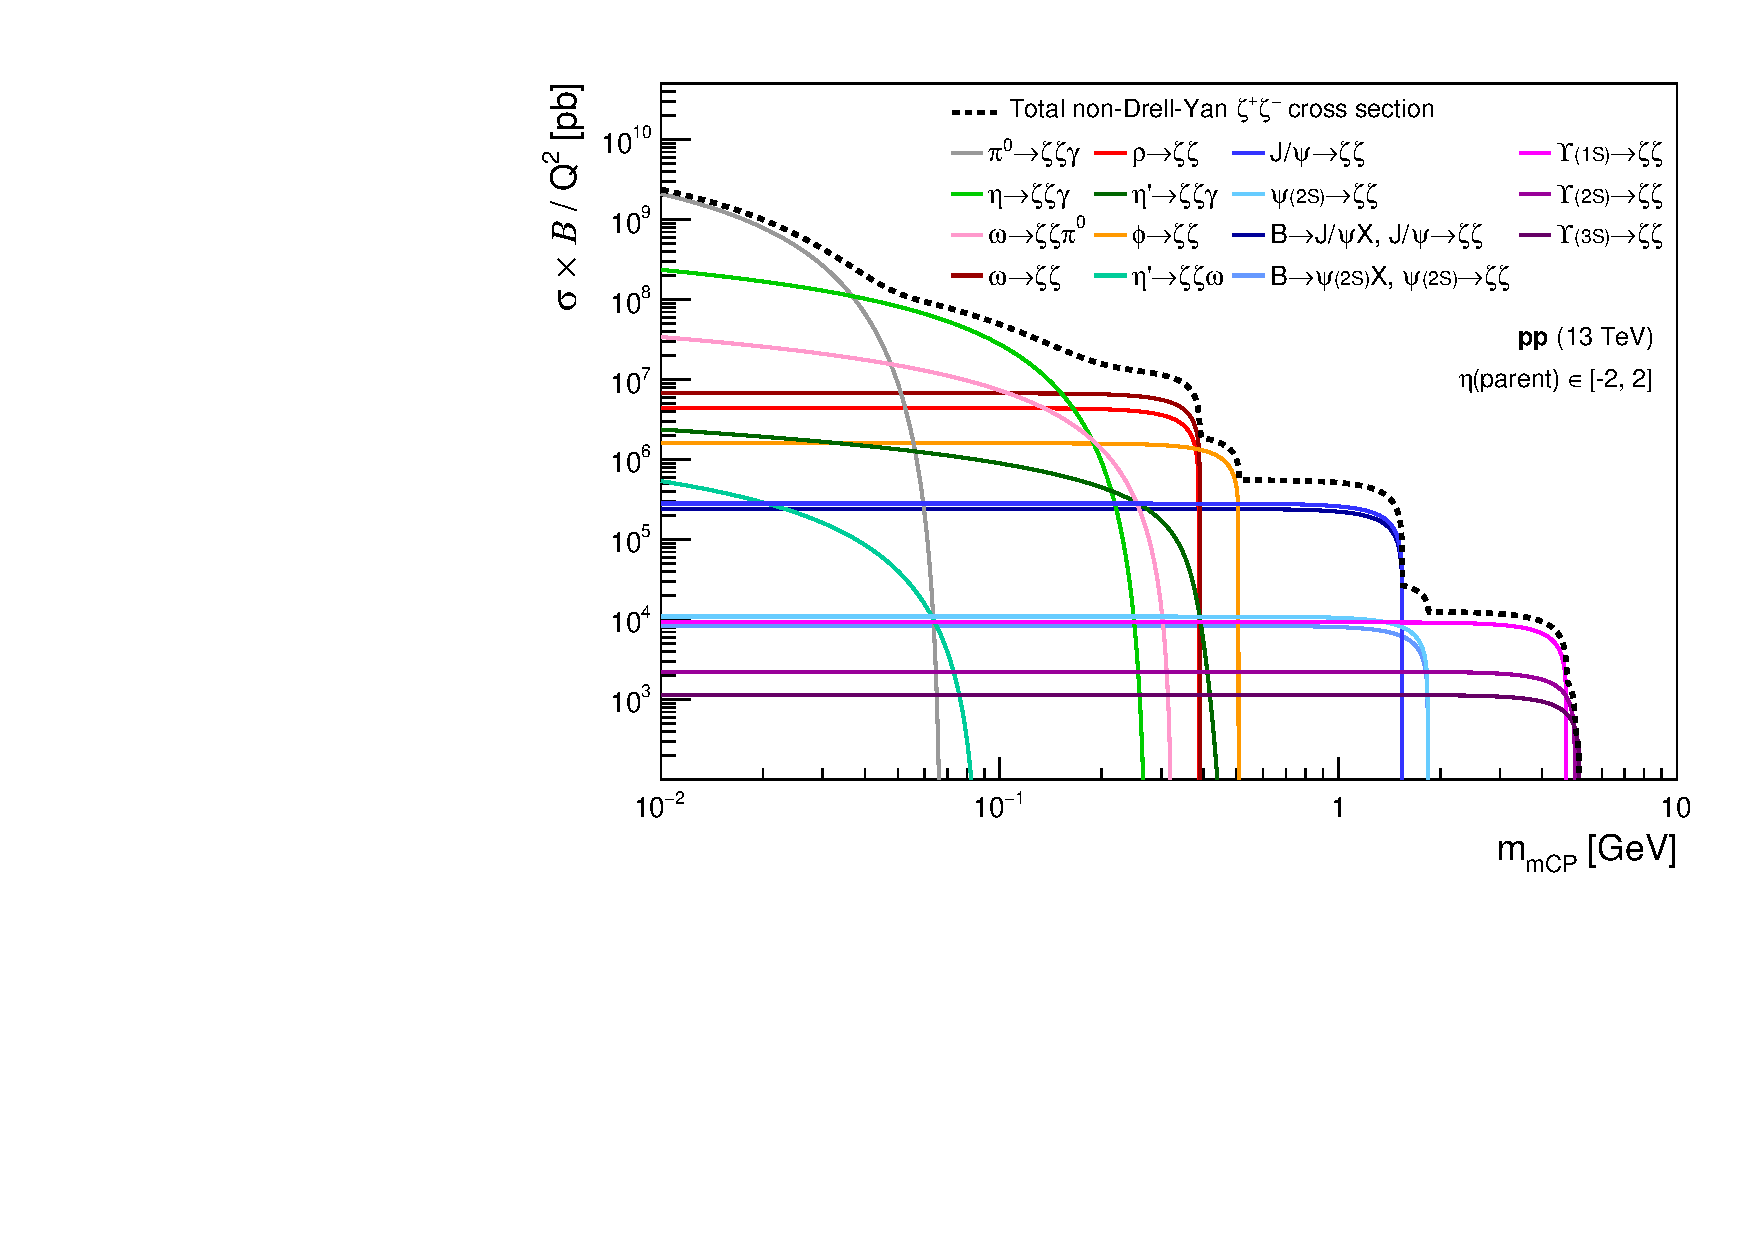
\includegraphics[width=0.8\linewidth]{../scripts/plot-xsecs/mcp-xsec.pdf}
  \caption{\protect Cross-section times branching ratios for various
    decays into $\zeta^+ \zeta^-$ pairs.  Note: this is
    the cross section for producing the mother particle times the
    branching ratio for the mother particle to decay into $\zeta^+ \zeta^-$.
    Multiply by two to get the $\zeta^{\pm}$ production cross section.
    For non-DY modes, the mother particle must be in $|\eta|<2$, but the
    daughter $\zeta^{\pm}$ could have $|\eta|>2$.  On the other hand some
    $\zeta$'s with $|\eta|<2$ can arise from mothers of $|\eta|>2$. For DY,
    it doesn't make sense to use ``mother $\eta$'' (it's almost always $\pm\infty$), 
    so the plotted cross section requires at least one mCP to have $|\eta|<1$. 
    This threshold was chosen so that the probability of an mCP pointing in the vicinity of 
    the detector is similar to that from the other non-DY production modes, 
    in order to facilitate comparison. The plateau in DY cross section below 
    $m_\zeta=1~\text{GeV}$ is due to a 2 GeV $\zeta^+\zeta^-$ invariant mass cut in MadGraph.}
\label{fig:total-rates}
\end{center}
  \end{figure}



As mentioned in the caption of Figure~\ref{fig:total-rates} some
of the $\zeta$'s in the central region (i.e.: potentially within
the acceptance of milliQan) could result from decays of mother
particles at higher $|\eta|$, especially in the cases where
the mother particles have low momentum and the boost in the
decay is small.
Particle production is
nearly flat in rapidity, see
Figures~\ref{fig:eta-upsilon},~\ref{fig:eta-psi}
for some examples.
The event generation will then
assume a flat pseudorapidity distribution.
At the analysis level one will be able to keep track of the
contributions from high $|\eta|$ mothers, and assign a systematic
if necessary.

\begin{figure}
  \begin{center}
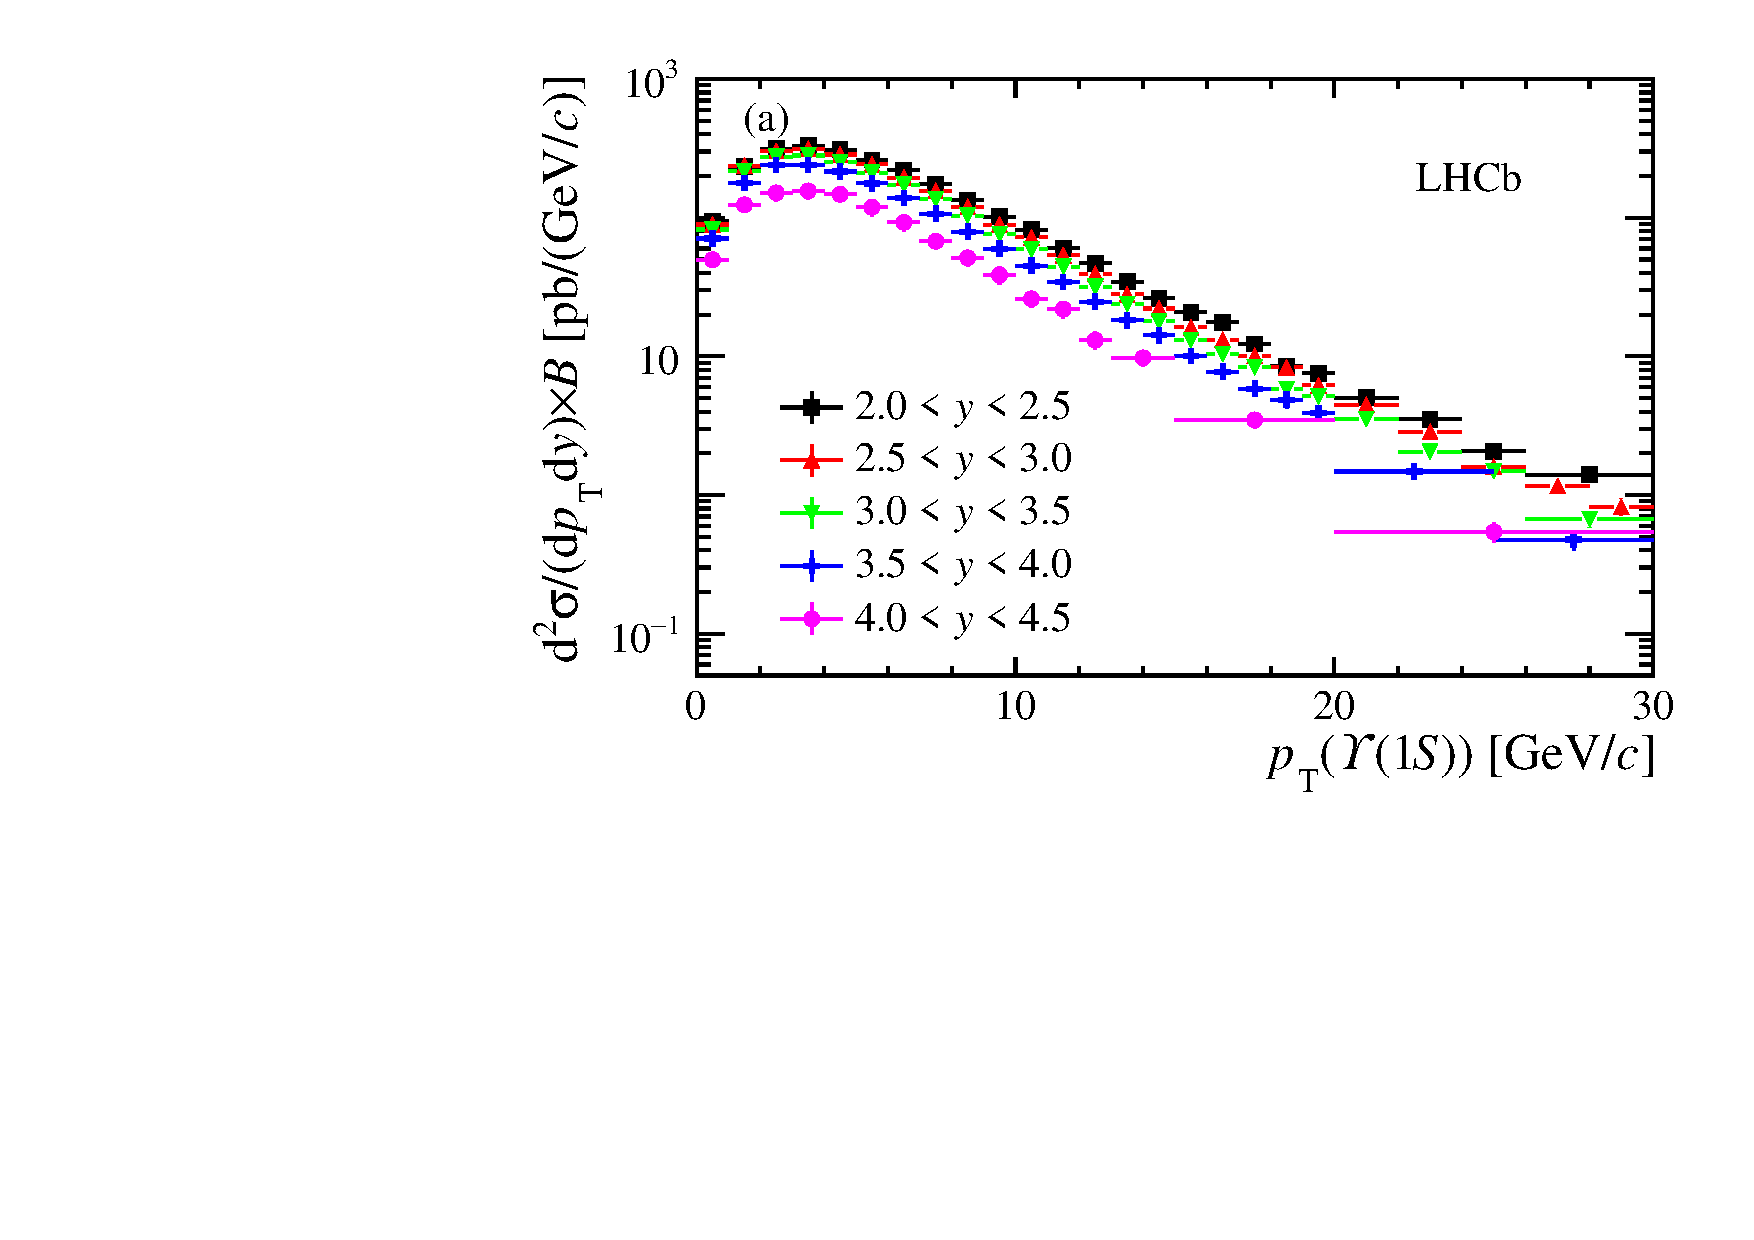
\includegraphics[width=0.5\linewidth]{plots/LHCb-eta.pdf}
\caption{\protect $\Upsilon(1S)$ spectra in different rapidity
  ranges from LHCb~\cite{Aaij:2018pfp}.}
    \label{fig:eta-upsilon}
\end{center}
  \end{figure}



\begin{figure}
\begin{adjustwidth}{-3cm}{-3cm}
\centering
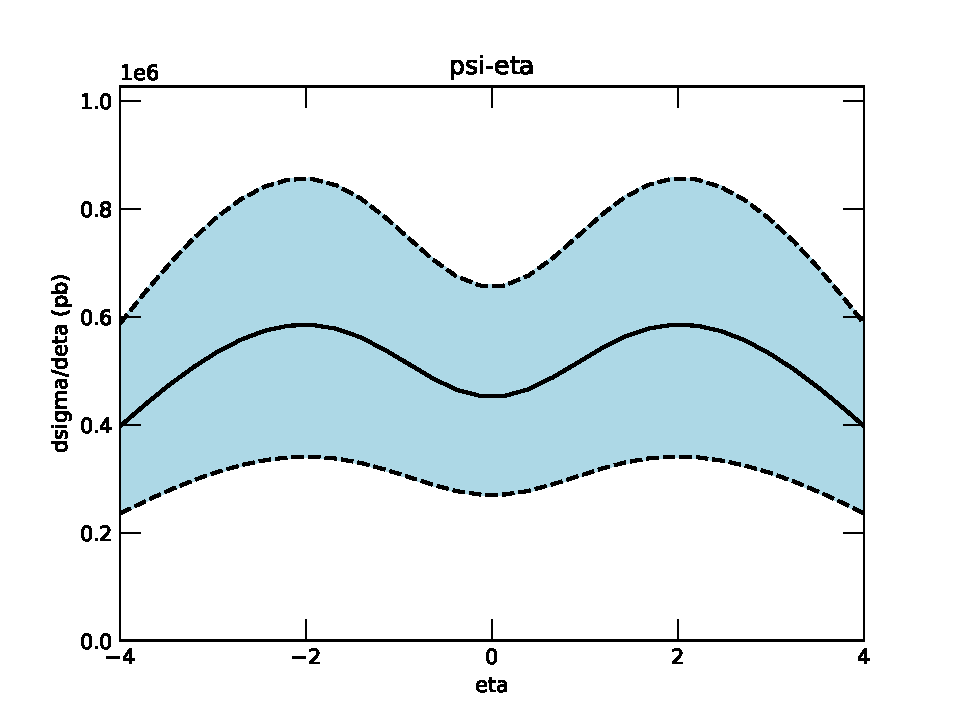
\includegraphics[width=0.22\linewidth]{../oniaFromB/psi-eta.pdf}
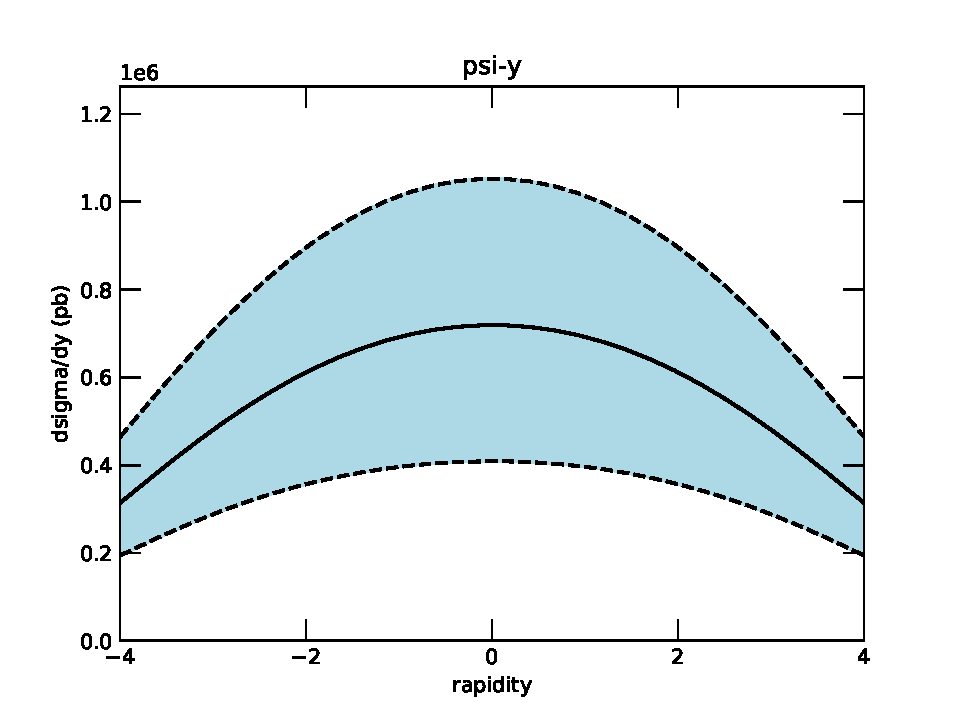
\includegraphics[width=0.22\linewidth]{../oniaFromB/psi-y.pdf}
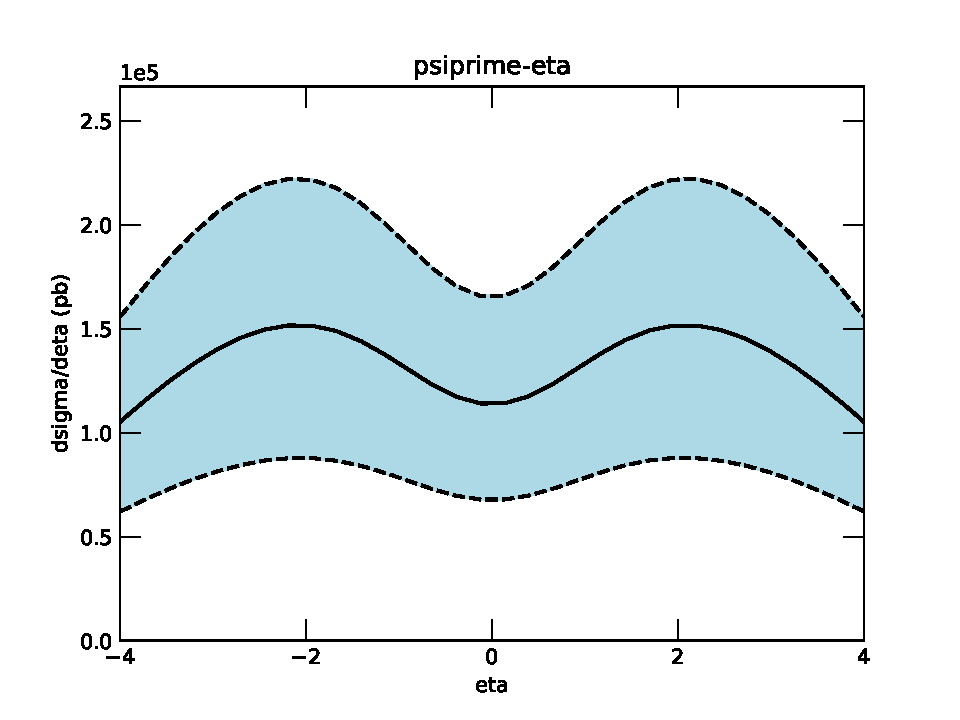
\includegraphics[width=0.22\linewidth]{../oniaFromB/psiprime-eta.pdf}
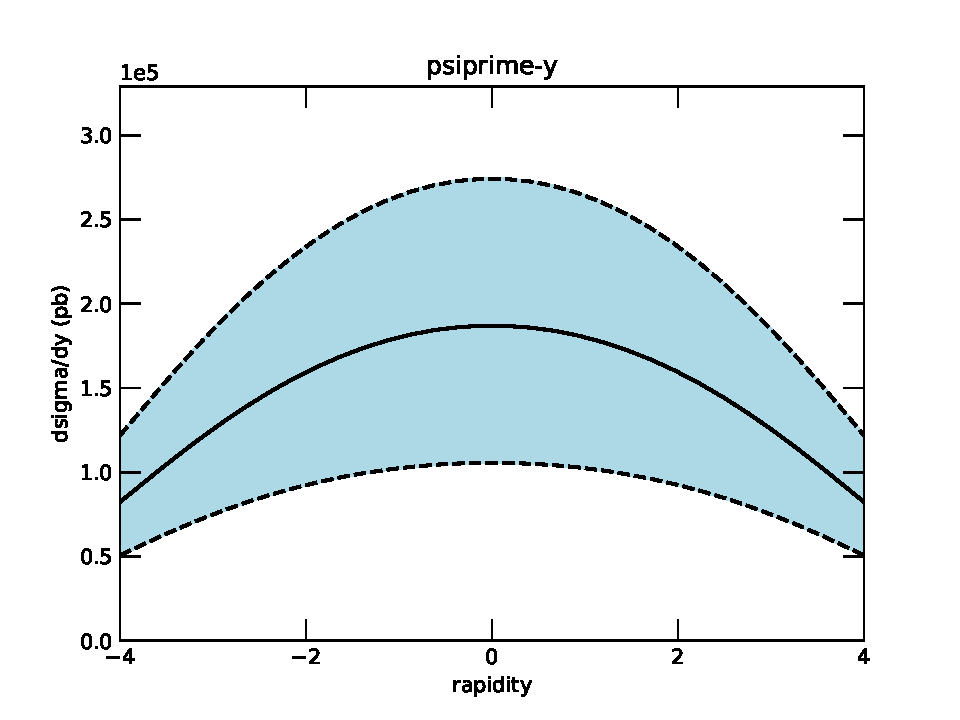
\includegraphics[width=0.22\linewidth]{../oniaFromB/psiprime-y.pdf}
\end{adjustwidth}
\caption{\protect Pseudorapidity and rapidity distributions
  from $\psi$ (left) and $\psi(2S)$ (right)
  from b-decays\cite{Cacciari:2012ny,Cacciari:2015fta}.
  These are for $p_T < 10$ GeV, i.e., in the low boost regime.
Note that in this $p_T$ range the theoretical uncertainties are large.}
  \label{fig:eta-psi}
\end{figure}








%%%%%%%%%%%%%%%%%%%%%%%%%%%%%%%%%%%%%%%%%%%%%%%%%%%%%%%%%%%%%%%%%%%%%%  
\clearpage
\section{Generation of the decays}

We provide functions that take as input the lab frame 4-vector of either pseudoscalar
($P$) or vector ($V$) meson, and return the 4 vectors of the two $\zeta$'s from the decay.
We assume that the $V$'s are unpolarized.


\subsection{Generation of pseudoscalar Dalitz decays}
The implementation goes as follows (this also works for the Dalitz
decay of the $\omega$, whcih has J=1,  as long as it is unpolarized):
\begin{itemize}
\item Rotate the 4-vector of $P$ from the lab frame into frame
  $S_1$ such that $P$ is traveling in the $z$-direction.
\item Boost along $z$ into frame $S_2$ where $P$ is at rest.
\item Pick a $q^2$ according to equation~\ref{dalitz1}.
\item Generate a decay $P \to X \gamma^*$ where $\gamma^*$ is
  a particle of $m^2 = q^2$.  The $\gamma^*$ direction is random
  in $\phi$ and random in $\cos \theta$.
\item Rotate the $\gamma^*$ 4-vector into a frame $S_3$ 
  such that the $\gamma^*$ is traveling in the $z$-direction.
\item Boost along $z$ into frame $S_4$ where $\gamma^*$ is at rest.
\item Generate a decay $\gamma^* \to \zeta^+ \zeta^-$ such that
  the angle $\phi$ of the $\zeta^+$ is random and
  $\cos \theta$ is picked according to~\cite{adlarson}
  \begin{equation}
    \frac{dN}{d \cos \theta} = 1 + \cos^2\theta + \frac{4 m^2_\zeta}{q^2} \sin^2\theta
    \label{dalitzAngles}
  \end{equation}
\item  Set the 3-vector of the $\zeta^-$ to be back-to-back with the $\zeta^+$.
\item Boost the 4-vectors of the $\zeta$'s from $S_4$ to $S_3$.
\item Rotate the 4-vectors of the $\zeta$'s from $S_3$ to $S_2$.
\item Boost the 4-vectors of the $\zeta$'s from $S_2$ to $S_1$.
\item Rotate the 4-vectors of the $\zeta$'s from $S_1$ to the lab frame.
\end{itemize}


\subsection{Generation of vector decays}

The procedure is the following:

\begin{itemize}
  \item Rotate the 4-vector of $V$ from the lab frame into frame
    $S_1$ such that $V$ is traveling in the $z$-direction.
  \item  Boost along $z$ into frame $S_2$ where $V$ is at rest.
  \item Generate a decay $V \to \zeta^+ \zeta^-$ such that
    both the angle $\phi$ and the $\cos \theta$ of the $\zeta^+$ are random.
  \item   Set the 3-vector of the $\zeta^-$ to be back-to-back with the $\zeta^+$.
  \item Boost the 4-vectors of the $\zeta$'s from $S_2$ to $S_1$.
\item Rotate the 4-vectors of the $\zeta$'s from $S_1$ to the lab frame.
\end{itemize}


\begin{thebibliography}{1}


\bibitem{Holdom}  B. Holdom, Phys.Lett. B166, 196 (1986).
  
%\cite{Haas:2014dda}
\bibitem{Haas:2014dda} 
  A.~Haas, C.~S.~Hill, E.~Izaguirre and I.~Yavin,
  %``Looking for milli-charged particles with a new experiment at the LHC,''
  Phys.\ Lett.\ B {\bf 746}, 117 (2015)
  doi:10.1016/j.physletb.2015.04.062
  [arXiv:1410.6816 [hep-ph]].
  %%CITATION = doi:10.1016/j.physletb.2015.04.062;%%
  %39 citations counted in INSPIRE as of 09 Jul 2019

%\cite{Ball:2016zrp}
\bibitem{Ball:2016zrp} 
  A.~Ball {\it et al.},
  %``A Letter of Intent to Install a milli-charged Particle Detector at LHC P5,''
  arXiv:1607.04669 [physics.ins-det].
  %%CITATION = ARXIV:1607.04669;%%
  %24 citations counted in INSPIRE as of 09 Jul 2019

  
\bibitem{landsberg}  L. G. Landsberg, Phys. Rep. 128, 301 (1985). 

\bibitem{bib:ulrik}
  See for example \href{http://cds.cern.ch/record/683210/files/soft-96-032.pdf}
{http://cds.cern.ch/record/683210/files/soft-96-032.pdf}.

\bibitem{VR1}
Aloni, D., Efrati, A., Grossman, Y. et al. J. High Energ. Phys. (2017) 2017: 19. 

\bibitem{VR2}
  R. Van Royen and V. F. Weisskopf, Nuovo Cim. A 50, 617 (1967) Erratum: [Nuovo Cim. A 51, 583 (1967)].

\bibitem{adlarson} P. Adlarson et al., Phys. Rev. C 95, 025202 (2007).

%\cite{Cacciari:2012ny,Cacciari:2015fta}
\bibitem{Cacciari:2012ny}
  M.~Cacciari, S.~Frixione, N.~Houdeau, M.~L.~Mangano, P.~Nason and G.~Ridolfi,
  % ``Theoretical predictions for charm and bottom
  % production at the LHC,''
  JHEP {\bf 1210} (2012) 137 [arXiv:1205.6344 [hep-ph]].
  %%CITATION = ARXIV:1205.6344;%%

\bibitem{Cacciari:2015fta}
  M.~Cacciari, M.~L.~Mangano and P.~Nason,
  %``Gluon PDF constraints from the ratio of forward heavy quark production at
  % the LHC at \sqrt{S}=7 and 13 TeV,''
  arXiv:1507.06197 [hep-ph].
  %%CITATION = ARXIV:1507.06197;%%

%\cite{Khachatryan:2010zg}
\bibitem{Khachatryan:2010zg} 
  V.~Khachatryan {\it et al.} [CMS Collaboration],
  %``Upsilon Production Cross-Section in pp Collisions at $sqrt{s}=7$ TeV,''
  Phys.\ Rev.\ D {\bf 83}, 112004 (2011)
  doi:10.1103/PhysRevD.83.112004
  [arXiv:1012.5545 [hep-ex]].
  %%CITATION = doi:10.1103/PhysRevD.83.112004;%%
  %143 citations counted in INSPIRE as of 22 Jun 2019

  %\cite{Chatrchyan:2013yna}
\bibitem{Chatrchyan:2013yna} 
  S.~Chatrchyan {\it et al.} [CMS Collaboration],
  %``Measurement of the $\Upsilon(1S), \Upsilon(2S)$, and $\Upsilon(3S)$ Cross Sections in $pp$ Collisions at $\sqrt{s}$ = 7 TeV,''
  Phys.\ Lett.\ B {\bf 727}, 101 (2013)
  doi:10.1016/j.physletb.2013.10.033
  [arXiv:1303.5900 [hep-ex]].
  %%CITATION = doi:10.1016/j.physletb.2013.10.033;%%
  %85 citations counted in INSPIRE as of 22 Jun 2019

%\cite{Khachatryan:2015qpa}
\bibitem{Khachatryan:2015qpa} 
  V.~Khachatryan {\it et al.} [CMS Collaboration],
  %``Measurements of the $\Upsilon$(1S), $\Upsilon$(2S), and $\Upsilon$(3S) differential cross sections in pp collisions at $\sqrt{s} =$ 7 TeV,''
  Phys.\ Lett.\ B {\bf 749}, 14 (2015)
  doi:10.1016/j.physletb.2015.07.037
  [arXiv:1501.07750 [hep-ex]].
  %%CITATION = doi:10.1016/j.physletb.2015.07.037;%%
  %36 citations counted in INSPIRE as of 22 Jun 2019


  %\cite{Sirunyan:2017qdw}
\bibitem{Sirunyan:2017qdw} 
  A.~M.~Sirunyan {\it et al.} [CMS Collaboration],
  %``Measurement of quarkonium production cross sections in pp collisions at $\sqrt{s}=$ 13 TeV,''
  Phys.\ Lett.\ B {\bf 780}, 251 (2018)
  doi:10.1016/j.physletb.2018.02.033
  [arXiv:1710.11002 [hep-ex]].
  %%CITATION = doi:10.1016/j.physletb.2018.02.033;%%
  %19 citations counted in INSPIRE as of 22 Jun 2019


  %\cite{Aad:2011xv}
\bibitem{Aad:2011xv}
  G.~Aad {\it et al.} [ATLAS Collaboration],
  %``Measurement of the $\Upsilon$(1S) production cross-section in $pp$ collisions at $\sqrt{s}=$ 7 TeV in ATLAS,''
  Phys.\ Lett.\ B {\bf 705} (2011) 9
  doi:10.1016/j.physletb.2011.09.092
  [arXiv:1106.5325 [hep-ex]].
  %%CITATION = doi:10.1016/j.physletb.2011.09.092;%%
  %44 citations counted in INSPIRE as of 22 Jun 2019

%\cite{Aad:2012dlq}
\bibitem{Aad:2012dlq} 
  G.~Aad {\it et al.} [ATLAS Collaboration],
  %``Measurement of Upsilon production in 7 TeV pp collisions at ATLAS,''
  Phys.\ Rev.\ D {\bf 87}, no. 5, 052004 (2013)
  doi:10.1103/PhysRevD.87.052004
  [arXiv:1211.7255 [hep-ex]].
  %%CITATION = doi:10.1103/PhysRevD.87.052004;%%
  %127 citations counted in INSPIRE as of 22 Jun 2019


%\cite{Aaij:2018pfp}
\bibitem{Aaij:2018pfp}
  R.~Aaij {\it et al.} [LHCb Collaboration],
  %``Measurement of $\Upsilon$ production in $pp$ collisions at $\sqrt{s}$= 13 TeV,''
  JHEP {\bf 1807} (2018) 134
   Erratum: [JHEP {\bf 1905} (2019) 076]
  doi:10.1007/JHEP07(2018)134, 10.1007/JHEP05(2019)076
  [arXiv:1804.09214 [hep-ex]].
  %%CITATION = doi:10.1007/JHEP07(2018)134, 10.1007/JHEP05(2019)076;%%
  %5 citations counted in INSPIRE as of 22 Jun 2019
  
  %\cite{Aaij:2015awa}
\bibitem{Aaij:2015awa}
  R.~Aaij {\it et al.} [LHCb Collaboration],
  %``Forward production of $\Upsilon$ mesons in $pp$ collisions at $\sqrt{s}=7$ and 8TeV,''
  JHEP {\bf 1511} (2015) 103
  doi:10.1007/JHEP11(2015)103
  [arXiv:1509.02372 [hep-ex]].
  %%CITATION = doi:10.1007/JHEP11(2015)103;%%
  %41 citations counted in INSPIRE as of 22 Jun 2019

  %\cite{Aaij:2014nwa}
\bibitem{Aaij:2014nwa}
  R.~Aaij {\it et al.} [LHCb Collaboration],
  %``Measurement of $\Upsilon$ production in $pp$ collisions at $\sqrt{s}=2.76$ TeV,''
  Eur.\ Phys.\ J.\ C {\bf 74} (2014) no.4,  2835
  doi:10.1140/epjc/s10052-014-2835-1
  [arXiv:1402.2539 [hep-ex]].
  %%CITATION = doi:10.1140/epjc/s10052-014-2835-1;%%
  %42 citations counted in INSPIRE as of 22 Jun 2019

  %\cite{Aaij:2013yaa}
\bibitem{Aaij:2013yaa} 
  R.~Aaij {\it et al.} [LHCb Collaboration],
  %``Production of J/psi and Upsilon mesons in pp collisions at sqrt(s) = 8 TeV,''
  JHEP {\bf 1306}, 064 (2013)
  doi:10.1007/JHEP06(2013)064
  [arXiv:1304.6977 [hep-ex]].
  %%CITATION = doi:10.1007/JHEP06(2013)064;%%
  %120 citations counted in INSPIRE as of 22 Jun 2019

%\cite{LHCb:2012aa}
\bibitem{LHCb:2012aa} 
  R.~Aaij {\it et al.} [LHCb Collaboration],
  %``Measurement of Upsilon production in pp collisions at $\sqrt{s}$ = 7 TeV,''
  Eur.\ Phys.\ J.\ C {\bf 72}, 2025 (2012)
  doi:10.1140/epjc/s10052-012-2025-y
  [arXiv:1202.6579 [hep-ex]].
  %%CITATION = doi:10.1140/epjc/s10052-012-2025-y;%%
  %127 citations counted in INSPIRE as of 22 Jun 2019

%\cite{Han:2014kxa}
\bibitem{Han:2014kxa} 
  H.~Han, Y.~Q.~Ma, C.~Meng, H.~S.~Shao, Y.~J.~Zhang and K.~T.~Chao,
  %``$\Upsilon(nS)$ and $\chi_b(nP)$ production at hadron colliders in nonrelativistic QCD,''
  Phys.\ Rev.\ D {\bf 94}, no. 1, 014028 (2016)
  doi:10.1103/PhysRevD.94.014028
  [arXiv:1410.8537 [hep-ph]].
  %%CITATION = doi:10.1103/PhysRevD.94.014028;%%
  %30 citations counted in INSPIRE as of 22 Jun 2019

%\cite{Ma:2010yw}
\bibitem{Ma:2010yw} 
  Y.~Q.~Ma, K.~Wang and K.~T.~Chao,
  %``$J/\psi (\psi^\prime)$ production at the Tevatron and LHC at ${\cal O}(\alpha_s^4v^4)$ in nonrelativistic QCD,''
  Phys.\ Rev.\ Lett.\  {\bf 106}, 042002 (2011)
  doi:10.1103/PhysRevLett.106.042002
  [arXiv:1009.3655 [hep-ph]].
  %%CITATION = doi:10.1103/PhysRevLett.106.042002;%%
  %204 citations counted in INSPIRE as of 27 Jun 2019  

  %\cite{Ma:2014mri}
\bibitem{Ma:2014mri} 
  Y.~Q.~Ma and R.~Venugopalan,
  %``Comprehensive Description of J/ψ Production in Proton-Proton Collisions at Collider Energies,''
  Phys.\ Rev.\ Lett.\  {\bf 113}, no. 19, 192301 (2014)
  doi:10.1103/PhysRevLett.113.192301
  [arXiv:1408.4075 [hep-ph]].
  %%CITATION = doi:10.1103/PhysRevLett.113.192301;%%
  %75 citations counted in INSPIRE as of 08 Aug 2019

  
%\cite{Ma:2010jj}
\bibitem{Ma:2010jj} 
  Y.~Q.~Ma, K.~Wang and K.~T.~Chao,
  %``A complete NLO calculation of the $J/\psi$ and $\psi'$ production at hadron colliders,''
  Phys.\ Rev.\ D {\bf 84}, 114001 (2011)
  doi:10.1103/PhysRevD.84.114001
  [arXiv:1012.1030 [hep-ph]].
  %%CITATION = doi:10.1103/PhysRevD.84.114001;%%
  %93 citations counted in INSPIRE as of 27 Jun 2019

%\cite{Khachatryan:2010yr}
\bibitem{Khachatryan:2010yr} 
  V.~Khachatryan {\it et al.} [CMS Collaboration],
  %``Prompt and Non-Prompt $J/\psi$ Production in $pp$ Collisions at $\sqrt{s}=7$ TeV,''
  Eur.\ Phys.\ J.\ C {\bf 71}, 1575 (2011)
  doi:10.1140/epjc/s10052-011-1575-8
  [arXiv:1011.4193 [hep-ex]].
  %%CITATION = doi:10.1140/epjc/s10052-011-1575-8;%%
  %254 citations counted in INSPIRE as of 08 Aug 2019

  
\bibitem{Sirunyan:2017zmn} 
  A.~M.~Sirunyan {\it et al.} [CMS Collaboration],
  %``Measurement of charged pion, kaon, and proton production in proton-proton collisions at $\sqrt{s}=13$ TeV,''
  Phys.\ Rev.\ D {\bf 96}, no. 11, 112003 (2017)
  doi:10.1103/PhysRevD.96.112003
  [arXiv:1706.10194 [hep-ex]].
  %%CITATION = doi:10.1103/PhysRevD.96.112003;%%
  %25 citations counted in INSPIRE as of 20 Jun 2019

\bibitem{CMS:tunes}
  A.~M.~Sirunyan {\it et al.} [CMS Collaboration],
  %``Event generator tunes obtained from underlying event and multiparton scattering measurements,''
  Eur. Phys. J. C (2016) 76: 155.
  doi:10.1140/epjc/s10052-016-3988-x
  [arXiv:1512.00815 [hep-ex]]
   
\bibitem{wwwPythia}
\href{http://home.thep.lu.se/\~torbjorn/pythia81php/Welcome.php}
{http://home.thep.lu.se/\~torbjorn/pythia81php/Welcome.php}.  Click on 
{\tt QCD} on the left panel.



  
\end{thebibliography}
  
\end{document}
